\documentclass[a4paper]{article}
\usepackage[T1]{fontenc}			% \chapter package
\usepackage[english]{babel}
\usepackage[english]{isodate}  		% date format
\usepackage{graphicx}				% manage images
\usepackage{amsfonts}
\usepackage{booktabs}				% high quality tables
\usepackage{amsmath}				% math package
\usepackage{amssymb}				% another math package (e.g. \nexists)
\usepackage{bm}                     % bold math symbols
\usepackage{mathtools}				% emphasize equations
\usepackage{stmaryrd} 				% '\llbracket' and '\rrbracket'
\usepackage{amsthm}					% better theorems
\usepackage{enumitem}				% manage list
\usepackage{pifont}					% nice itemize
\usepackage{cancel}					% cancel math equations
\usepackage{caption}				% custom caption
\usepackage[]{mdframed}				% box text
\usepackage{multirow}				% more lines in a table
\usepackage{textcomp, gensymb}		% degree symbol
\usepackage[x11names]{xcolor}		% RGB color
\usepackage[many]{tcolorbox}		% colorful box
\usepackage{multicol}				% more rows in a table (used for the lists)
\usepackage{listings}
\usepackage{url}
\usepackage{qrcode}
\usepackage{fontawesome5}
\usepackage{ragged2e}
\usepackage{cite}                   % references
\usepackage{imakeidx}               % index
\makeindex[program=makeindex, columns=1,
           title=Index, 
           intoc,
           options={-s index-style.ist}]


\definecolor{codegreen}{rgb}{0,0.6,0}
\definecolor{codegray}{rgb}{0.5,0.5,0.5}
\definecolor{codepurple}{rgb}{0.58,0,0.82}
\definecolor{backcolour}{rgb}{0.95,0.95,0.92}
\lstdefinestyle{mystyle}{
    backgroundcolor=\color{backcolour},   
    commentstyle=\color{codegreen},
    keywordstyle=\color{magenta},
    numberstyle=\tiny\color{codegray},
    stringstyle=\color{codepurple},
    basicstyle=\ttfamily\footnotesize,
    breakatwhitespace=false,         
    breaklines=true,                 
    captionpos=b,                    
    keepspaces=true,                 
    numbers=left,                    
    numbersep=5pt,                  
    showspaces=false,                
    showstringspaces=false,
    showtabs=false,                  
    tabsize=2
}
\lstset{style=mystyle}


% draw a frame around given text
\newcommand{\framedtext}[1]{%
	\par%
	\noindent\fbox{%
		\parbox{\dimexpr\linewidth-2\fboxsep-2\fboxrule}{#1}%
	}%
}


% table of content links
\usepackage{xcolor}
\usepackage[linkcolor=black, citecolor=blue, urlcolor=cyan]{hyperref} % hypertexnames=false
\hypersetup{
	colorlinks=true
}


\newtheorem{theorem}{\textcolor{Red3}{\underline{Theorem}}}
\renewcommand{\qedsymbol}{QED}
\newcommand{\dquotes}[1]{``#1''}
\newcommand{\longline}{\noindent\rule{\textwidth}{0.4pt}}
\newcommand{\circledtext}[1]{\raisebox{.5pt}{\textcircled{\raisebox{-.9pt}{#1}}}}
\newcommand{\definition}[1]{\textcolor{Red3}{\textbf{#1}}\index{#1}}
\newcommand{\example}[1]{\textcolor{Green4}{\textbf{#1}}}
\newcommand{\highspace}{\vspace{1.2em}\noindent}


\begin{document}
    \newcounter{definition}[section]
    \newcounter{example}[section]
    
    \newtcolorbox[use counter = definition]{definitionbox}[1][]{%
        colback=red!5!white,
        colframe=red!75!black,
        fonttitle=\bfseries,
        title={Definition \thetcbcounter #1} %
    }
    
    \newtcolorbox[use counter = example]{examplebox}[1][]{%
        breakable,
        enhanced,
        colback=Green4!5!white,
        colframe=Green4!75!black,
        fonttitle=\bfseries,
        title={Example \thetcbcounter #1} %
    }

    %%%%%%%%%%%%%%%
    % Notes cover %
    %%%%%%%%%%%%%%%
    \author{260236}
\title{Software Engineering for HPC - Notes}
\date{\printdayoff\today}
\maketitle

    %%%%%%%%%%%
    % Preface %
    %%%%%%%%%%%
    \section*{Preface}

Every theory section in these notes has been taken from two sources:
\begin{itemize}
    \item None
\end{itemize}
About:
\begin{itemize}
    \item[\faIcon{github}] \href{https://github.com/PoliMI-HPC-E-notes-projects-AndreVale69/HPC-E-PoliMI-university-notes}{GitHub repository}
\end{itemize}
    
    %%%%%%%%%%%%%%%%%%%%%
    % Table of contents %
    %%%%%%%%%%%%%%%%%%%%%
	\tableofcontents

    %%%%%%%%%%%%%%%%
    % Introduction %
    %%%%%%%%%%%%%%%%
    \section{Software Configuration Management}

\subsection{Introduction}

\href{https://www.atlassian.com/microservices/microservices-architecture/configuration-management}{Configuration Management (CM)} is a systems engineering process for establishing consistency of a product's attributes throughout its life. In the technology world, configuration management is an IT management process that tracks individual configuration items of an IT system. IT systems are composed of IT assets that vary in granularity. An IT asset may represent a piece of software, or a server, or a cluster of servers. The following focuses on configuration management as it directly applies to IT software assets and software asset CI/CD.

\highspace
\definition{Software Configuration Management} is a \textbf{systems engineering process that tracks and monitors changes to a software systems configuration metadata}. In software development, configuration management is commonly used alongside version control and CI/CD infrastructure (explained later).

\highspace
The basic \textbf{approach to using a decentralized CM} is to have a repository (project) on the server side. 
\begin{itemize}
    \item When we want to work on the project, we clone the repository on the local PC. This workflow is used because we can work offline and on the local project without making critical changes to the repository server side.
    
    \item The local changes can be saved using the commit command and when we are ready to publish our changes, we use the push command to update the repository on the server side.
    
    \item After a push, anyone who has a local copy should make a pull command to update the local project.
\end{itemize}
This workflow can be done using git commands, and a good cheat sheet can be found \href{https://education.github.com/git-cheat-sheet-education.pdf}{here}.
    
    %%%%%%%%%%%%%%%%%%%%%%%%%%%%%%%%%%%%%%%%%%%%%%%%%%%%%%%%%%%%%%%%%%%
    % HPC Software, Relevant Qualities and System Engineering Methods %
    %%%%%%%%%%%%%%%%%%%%%%%%%%%%%%%%%%%%%%%%%%%%%%%%%%%%%%%%%%%%%%%%%%%
    \section{HPC Software, Relevant Qualities and Systems Engineering Methods}

\subsection{High Performance Computing Software}

There's no single definition of HPC, but it can be explained in a number of ways:
\begin{definitionbox}
    The practice of aggregating computing power in a way that delivers much high performance than one could get out of a typical desktop computer or workstation to solve large problems in science, engineering, or business.

    \highspace
    Thousands of processors working in parallel to analyze billions of pieces of data in real time, performing calculations thousands of times faster than a normal computer.

    \highspace
    The use of parallel processing for running advanced, large-scale application programs efficiently, reliably and very quickly on supercomputer systems.

    \highspace
    The platform technology concerned with programming for performance, where performance takes the broad meaning of:
    \begin{itemize}
        \item Speed (reducing time to solution);
        \item Energy efficiency (doing more with less power);
        \item Upscaling (handling larger problems such as simulating a wing aand then a full plane, or a cell and then an organ);
        \item High throughput (the ability to handle large volumes of data in near real-time, as required in the financial services industry, telecoms or satellite imagery).
    \end{itemize}
\end{definitionbox}

\noindent
As \definition{Parallel and Distributed Computing (PDC)} exist, it is necessary to explain the difference. The main characteristics of PDC are:
\begin{itemize}
    \item \textbf{Concurrency}: it is a property of software. \textbf{A piece of software is also concurrent if it can have more than one active execution context}.

    \item \textbf{Parallelism}: it is a property of software. \textbf{The execution of different tasks/pieces of software at the same time}.

    \item \textbf{Distribution}. \textbf{The execution of different tasks/pieces of software on physically distinct computing nodes connected through a network, lack of a global clock}.
\end{itemize}
\textbf{PDCs} are \textbf{multi-core machines}, whereas \textbf{HPCs} are \textbf{quantum computers}. However, \textbf{both share parallel machines}, \textbf{HPC clusters} and \textbf{cloud infrastructures}.

\newpage

\noindent
There are \textbf{two categories} of HPC software:
\begin{itemize}
    \item \definition{Compute-intensive applications}. These are \textbf{complex calculations that require a large number of computing resources}. They also often require parallel computing.

    \item \definition{Data-intensive applications}. They \textbf{focus on processing, storing and retrieving large amounts of data}. Typically built as distributed systems to ensure reliability and scalability.
\end{itemize}
    \subsection{Relevant Qualities}

For the two categories explained, there are some important characteristics:
\begin{itemize}
    \item For \definition{Compute-intensive applications}:
    \begin{itemize}
        \item \underline{\definition{Correctness}}: the \textbf{software is correct if it satisfies the specifications}, but be careful! Sometimes, modelling reality into a model (using the specifications) isn't the bigger problem. Instead, it is difficult or impossible to show actual correctness concerning reality. For \example{example}, imagine you are building a simulator of a planet lander before you have ever visited it.
        
        \emph{How can you fix this issue?} We can \textbf{check that the software output fulfils the important desired properties} and \textbf{identify and apply a measure of accuracy}.

        
        \item \underline{\definition{Performance}}: it is the \textbf{efficient use of resources}. Again, be careful! Is it a good idea? Is performance improvement always a good idea? Because it is \textbf{not necessarily if}:
        \begin{itemize}
            \item It makes software \textbf{more difficult to read} and \textbf{maintain}
            \item It \textbf{reduces the portability} of software
        \end{itemize}
        
        
        \item \underline{\definition{Portability}}.
        
        
        \item \underline{\definition{Maintainability}}. A system can have this feature if it follows \textbf{three principles}:
        \begin{enumerate}
            \item \definition{Operability}: \textbf{make it easy for the operations team to run the system and keep it running}. There are a number of things that need to be done to achieve this:
            \begin{itemize}
                \item Provide visibility into the runtime behavior and internals of the system, with good monitoring.

                \item Provide good support for automation and integration with standard tools.

                \item Avoidance of dependencies on individual machines (allowing machines to be taken down for maintenance while the system as a whole continues to run uninterrupted).

                \item Provide good documentation and an easy to understand operational model (\dquotes{If I do X, Y will happen}).

                \item Provide good default behavior, but also give administrators the freedom to override defaults when necessary.

                \item Self-healing when appropriate, but also giving administrators manual control over system state when needed.
            \end{itemize}
            
            \item \definition{Simplicity}: \textbf{make it easy for other software engineers to understand the system}. This is necessary because complex systems take more time to understand and increase the cost of maintenance. There are several techniques for doing this:
            \begin{itemize}
                \item Reducing \emph{accidental complexity}.
                
                \item Using abstractions, such as organising the architecture into well-defined components that hide the internal complexity behind a clear and easy-to-use interface; or reusing known solutions.
            \end{itemize}

            \item \definition{Evolvability}: make it easy for engineers to change the system as new requirements emerge. There are a number of things that need to be done to achieve this:
            \begin{itemize}
                \item Organize your development process to cope with evolution.
                
                \item Keep track of how requirements are mapped to your software structure.

                \item Update documentation.

                \item Continue to ensure simplicity and operability.
            \end{itemize}
        \end{enumerate}
    \end{itemize}

    \item For \definition{Data-intensive applications}:
    \begin{itemize}
        \item \underline{\definition{Reliability}}: can be mathematically defined as \textbf{probability of absence of failures for a certain period}. The typical expectations are:
        \begin{itemize}
            \item The application \textbf{performs the expected function}
            \item It can \textbf{tolerate mistakes by users}
            \item It \textbf{prevents unauthorized access} and \textbf{abuse}
        \end{itemize}
        
        
        \item \underline{\definition{Scalability}}: the \textbf{system ability to cope with increased load}. The load unit depends on the product: for web apps can be represented with the number of requests per second; for databases can be the number of read and write operation (or their ratio).
        
        
        \item \underline{\definition{Maintainability}}. Same as above.
    \end{itemize}
\end{itemize}
In the software, there can be some errors, but a software engineer should be able to recognize the type of failure, faults or defects:
\begin{itemize}
    \item A \definition{defect} is an \textbf{imperfection or deficiency in a work product} where that work product does \underline{not meet its requirements or specifications} and needs to be either repaired or replaced.

    \item A \textbf{defect encountered during software execution} is a \definition{fault} (a fault is a subtype of defect, and can be of two types, see below).
    
    \item A \definition{system failure} can be:
    \begin{itemize}
        \item Termination of the ability of a product to perform a required function or its inability to perform within previously specified limits.

        \item An event in which a system or system component does not perform a required function within specified limits.
    \end{itemize}
\end{itemize}
There are some exceptions where systems are \definition{fault-tolerant} or \definition{resilient}. These are systems that can \textbf{cope with faults and prevent faults from occurring}. An \textbf{advantage of fault-tolerance} is that \textbf{reliability is increased}. 

\newpage

\noindent
The \textbf{fault} can be of \textbf{two types}:
\begin{itemize}
    \item \definition{Hardware Faults}.
    \begin{flushleft}
        \textcolor{Red2}{\textbf{\faIcon{exclamation-triangle} Description of the problem}}
    \end{flushleft}
    It is a defect encountered during hardware execution. In a large datacenter these can happen on a daily basis. Different pieces of hardware usually fail independently from each other.
    \begin{flushleft}
        \textcolor{Green3}{\textbf{\faIcon{check} Possible solutions}}
    \end{flushleft}
    The possible solutions are two: \textbf{hardware redundancy} and \textbf{software fault-tolerance techniques}.

    \item \definition{Software Faults}.
    \begin{flushleft}
        \textcolor{Red2}{\textbf{\faIcon{exclamation-triangle} Description of the problem}}
    \end{flushleft}
    They result from \textbf{software development errors}. Can stay dormant for a long time and appear suddenly. They can \textbf{determine failures in multiple components} at the same time.
    \begin{flushleft}
        \textcolor{Green3}{\textbf{\faIcon{check} Possible solutions}}
    \end{flushleft}
    There is no single solution! It is a combination of strategies. So use defensive programming, by testing before release and during operation:
    \begin{itemize}
        \item Reboot the system frequently (rejuvenation)
        \item Continuous monitoring and alerting in case of possible symptoms
        \item Deliberately introduce failures to train the fault tolerance machinery (chaos engineering)
    \end{itemize}
\end{itemize}

\longline

\subsection{Systems Engineering Methods}

There are several systems engineering methodologies required in High Performance Computing:
\begin{itemize}
    \item Modelling the software structure and checking its properties.
    
    \item Performance analysis and improvement.
    
    \item Source code management.
    
    \item Documentation, standards, support to maintainability.
    
    \item Support to scalability.
    
    \item Attention to operability and automation.
\end{itemize}

    %%%%%%%%%%%%%%%%%%%%%%%%%%%
    % Requirement Engineering %
    %%%%%%%%%%%%%%%%%%%%%%%%%%%
    \section{Requirement Engineering}

\subsection{Definition}

Before the definition, we give a possible scenario to understand what requirement engineering is.

\highspace
The municipality of Milan says the following: \dquotes{\emph{The time it takes to make decisions on building permits for residential buildings in the city is too long. We want to develop software that will help us reduce this time}}. So where do we start? How do we identify the most important aspects? How do we make sure that we have understood what our customers want from us?

\begin{definitionbox}
    Software measure engineering (\definition{Requirement Engineering}) is the process of discovering the purpose for which the software is intended by identifying stakeholders and their needs, and documenting these in a form suitable for analysis, communication and subsequent implementation.
\end{definitionbox}

\noindent
The questions derived from requirements engineering are:
\begin{itemize}
    \item Identify stakeholders
    \item Identify their needs
    \item Produce documentation
    \item Analyze, communicate, implement requirements
\end{itemize}

\begin{figure}[!htp]
    \centering
    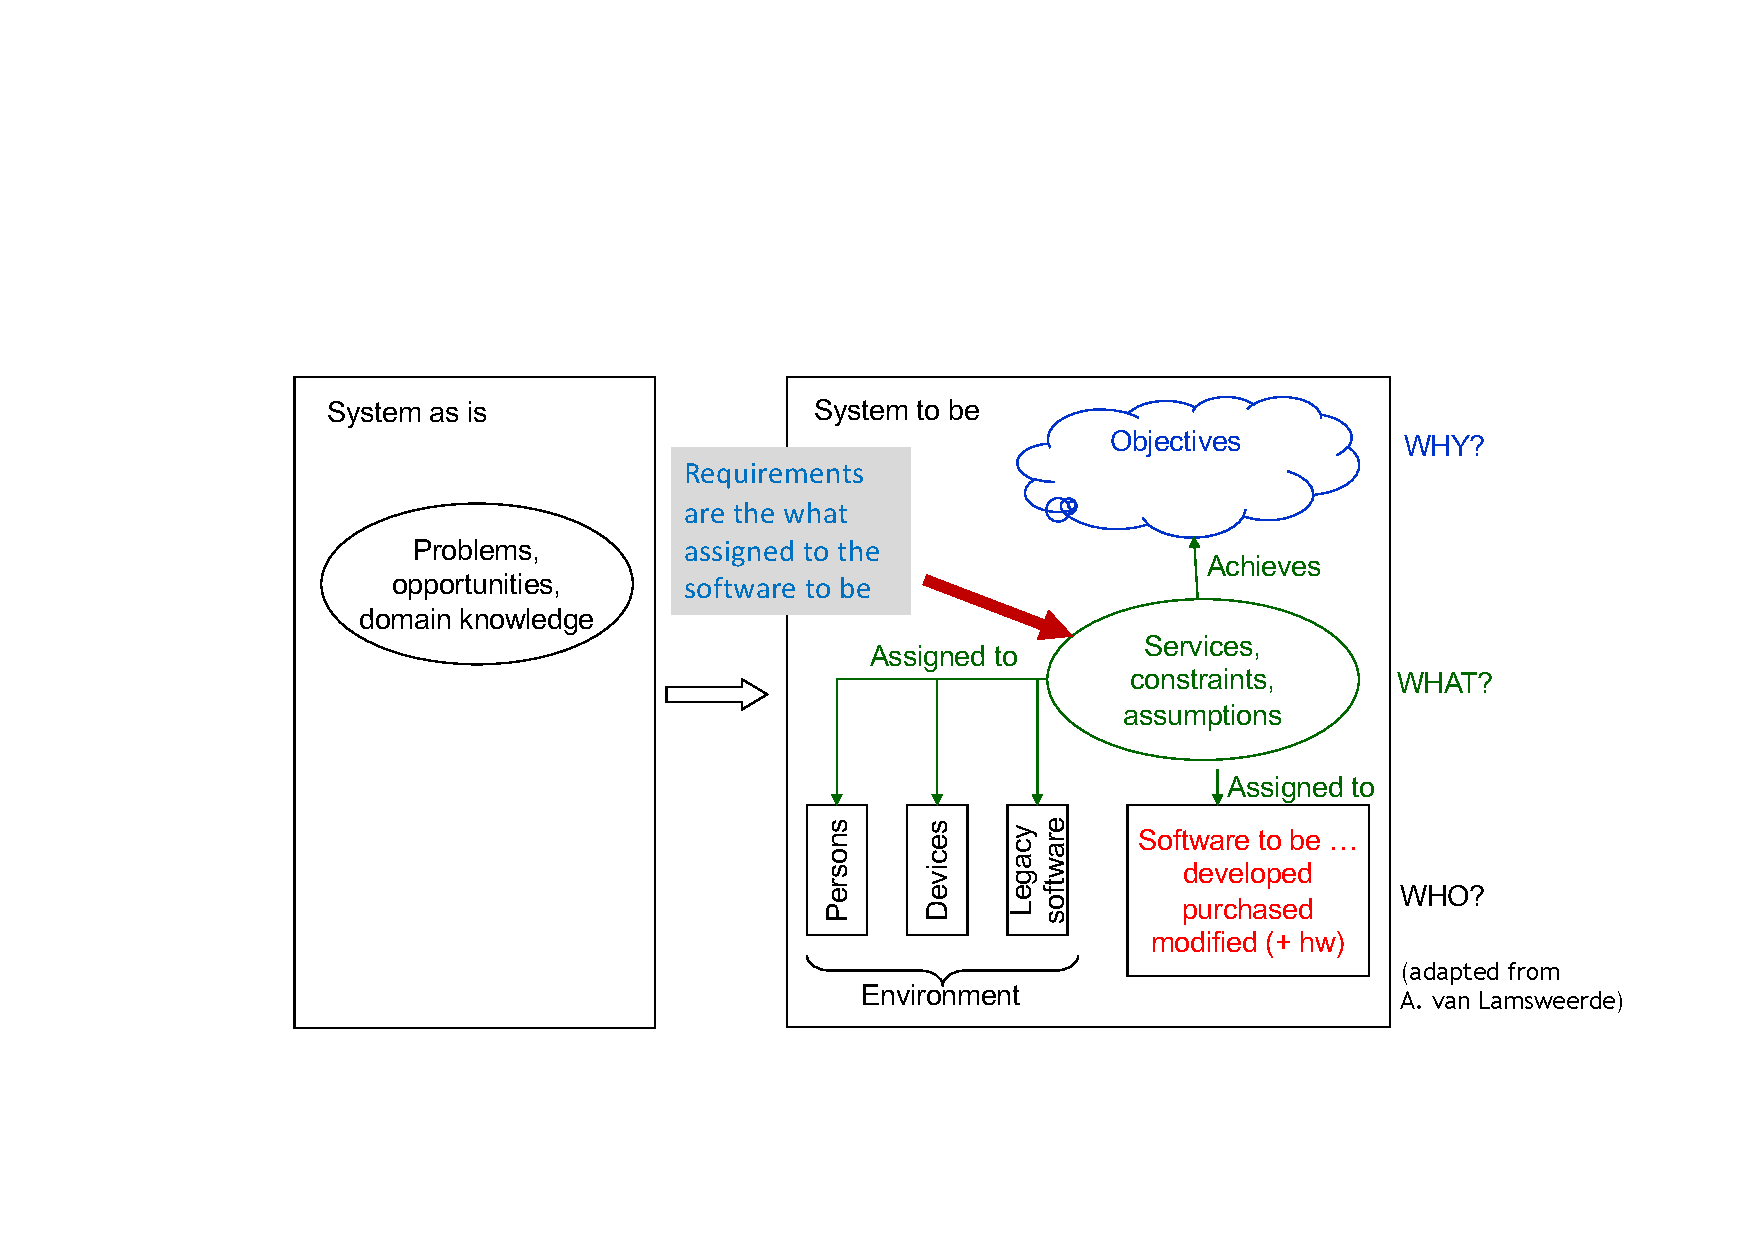
\includegraphics[width=\textwidth]{img/requirement-engineering-1.pdf}
    \caption{Analyzing the system as is and the system to be.}
\end{figure}
    \subsection{Studying the interplay between the world and the machine}

\begin{examplebox}[: ambulance dispatching system]\label{example: ambulance dispatching system}
    For every urgent call reporting an incident, an ambulance should arrive at the incident location within 14 minutes. For every urgent call, details about the incident are correctly encoded.

    When an ambulance is dispatched, it will reach the incident location in the shortest possible time. Accurate ambulance locations are known by GPS. Ambulance crews correctly notify ambulance availability through a mobile data terminal.

    \highspace
    Given the previous problem, are you able to extract requirements from this description? Some possible questions might be:
    \begin{itemize}
        \item Should the software system drive the ambulance?

        \item Who or what will \dquotes{correctly encode} details about incidents?
        
        \item Do terminals already exist or not?
    \end{itemize}
    And more in general:
    \begin{itemize}
        \item What are the boundaries of the system? What is inside/outside? What is in-between?

        \item How do we think about these aspects in a systematic way?
    \end{itemize}
\end{examplebox}

\noindent
This example is necessary to understand the \textbf{phenomena of world and machine}. The \definition{machine} \textbf{is the part of the system to be developed} (typically a software-to-be and a hardware). The \definition{world} (or environment) \textbf{is the part of the real world that is affected by the machine}.

\highspace
Requirements engineering is \textbf{concerned with the phenomena that occur in the world}. In the previous \example{example}, RE is concerned with the following phenomena:
\begin{itemize}
    \item Occurrence of incidents
    \item Reports of incidents by public calls
    \item Encoding of call details into dispatching software
    \item Assignment of an ambulance
    \item Arrival of an ambulance at the scene of an incident
\end{itemize}
But RE is also interested in the phenomena that occur inside the machine. In the previous \example{example}
\begin{itemize}
    \item The creation of a new object of the class \texttt{Incident}
    \item The updating of a database entry
\end{itemize}
\textbf{Requirements models are models of the world!}

\newpage

\noindent
Using the \example{example} on the previous page, we can show the phenomena we are interested in the world or in the machine set.
\begin{figure}[!htp]
    \centering
    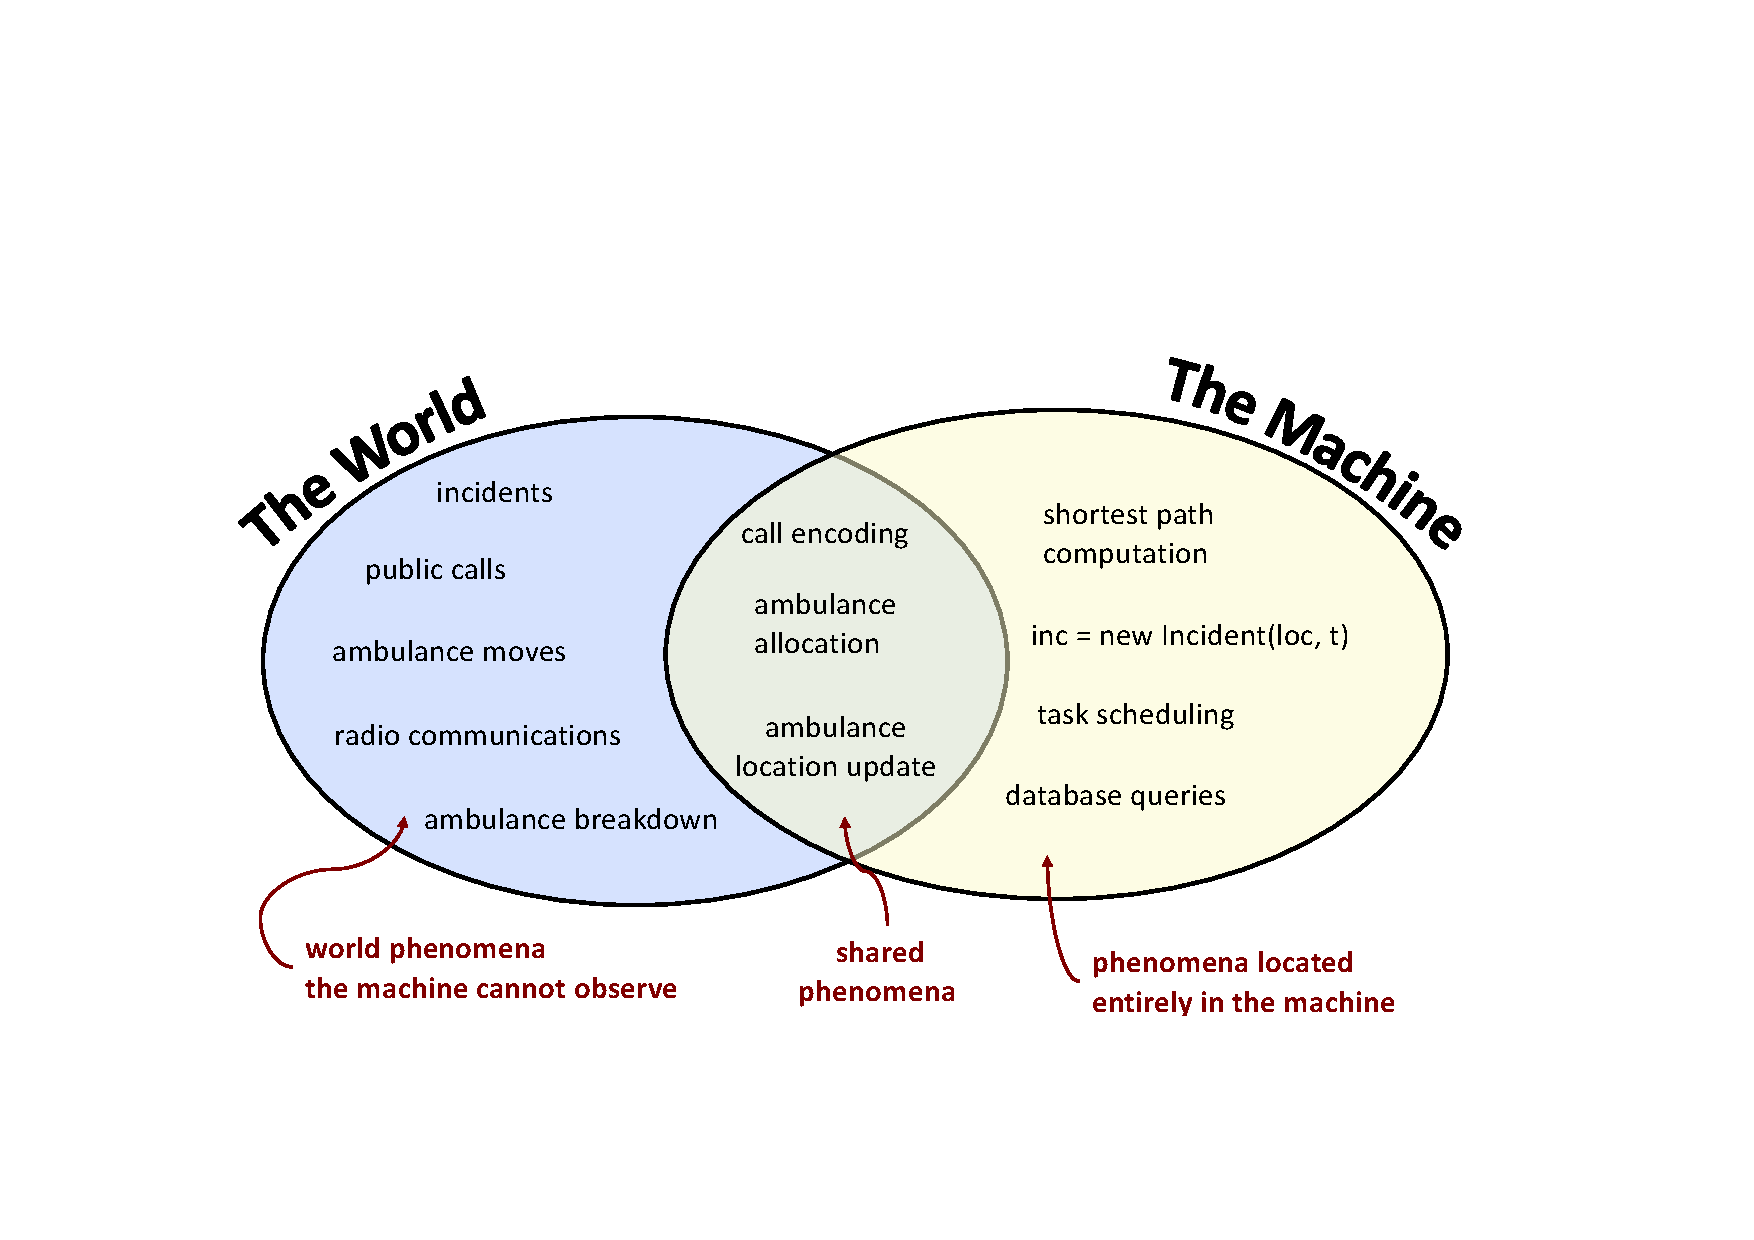
\includegraphics[width=\textwidth]{img/world-and-machine-1.pdf}
    \caption{The world and the machine sets, with reference to example on page~\pageref{example: ambulance dispatching system}.}
\end{figure}

\noindent
More generally, we can divide the machine and the world sets as:
\begin{itemize}
    \item The world which have goals and domain properties;
    \item The machine which have computers and programs;
    \item The requirements which is the bridge between the world and the machine.
\end{itemize}

\begin{figure}[!htp]
    \centering
    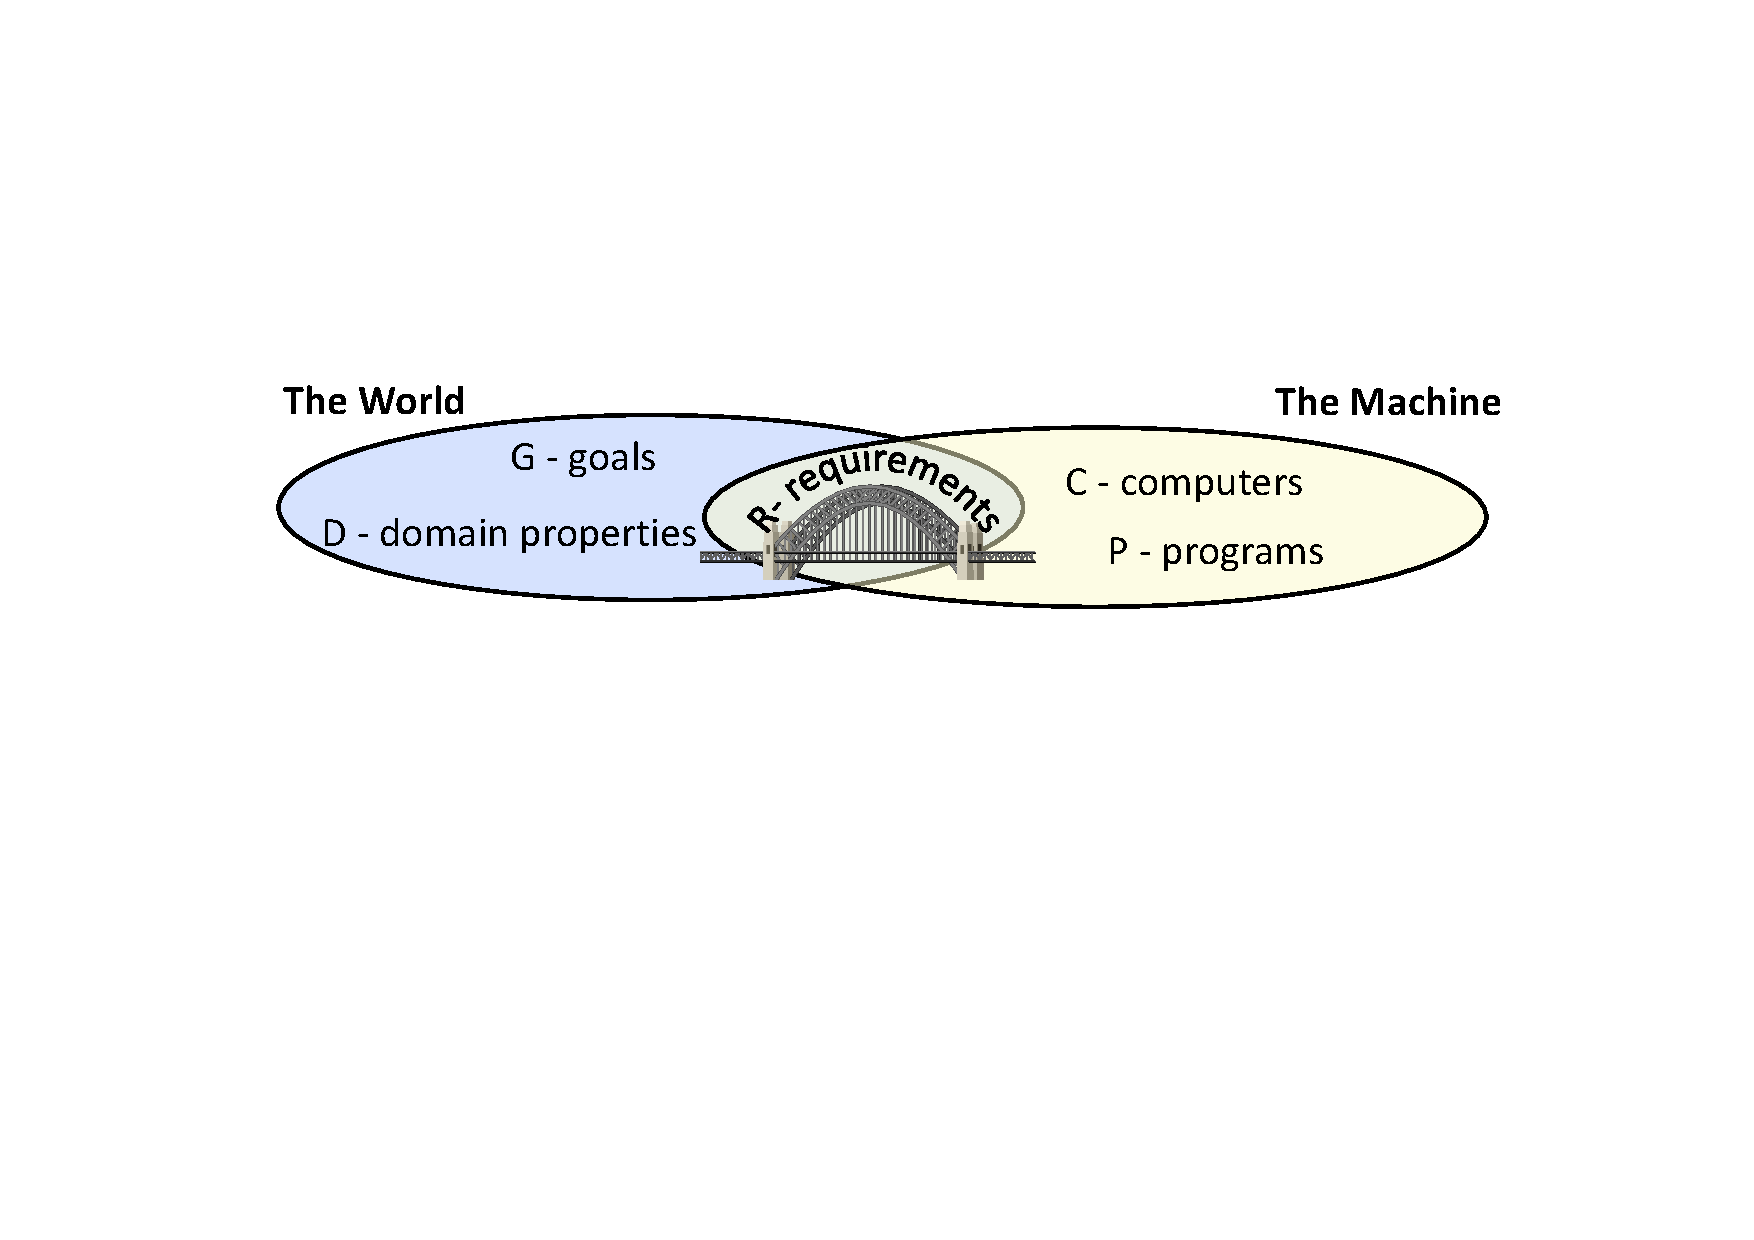
\includegraphics[width=\textwidth]{img/world-and-machine-2.pdf}
    \caption{Goals, domain properties, requirements, computers and programs.}
\end{figure}

\noindent
We explain more detailed these value inside the two sets:
\begin{itemize}
    \item \definition{Goals} are \textbf{prescriptive assertions formulated in terms of world phenomena} (not necessarily shared)
    \item \definition{Domain properties} (or assumptions) are \textbf{descriptive assertions assumed to hold in the world}
    \item \definition{Requirements} are \textbf{prescriptive assertions formulated in terms of shared phenomena} 
\end{itemize}

\newpage

\noindent
Using the \example{example} on the page~\pageref{example: ambulance dispatching system}, we can identify the goal, the domain assumptions and the requirement as follows:
\begin{itemize}
    \item \textbf{Goal}: \emph{For every urgent call reporting an incident, an ambulance should arrive at the incident scene within 14 minutes}.

    \item \textbf{Domain assumptions}:
    \begin{itemize}
        \item \emph{For every urgent call, details about the incident are correctly encoded}.
        \item \emph{When an ambulance is mobilized, it will reach the incident location in the shortest possible time}.
        \item \emph{Accurate ambulances' location are known by GPS}.
        \item \emph{Ambulance crews correctly signal ambulance availability through mobile data terminals on board of ambulances}.
    \end{itemize}
    
    \item \textbf{Requirement}: \emph{When a call reporting a new incident is encoded, the Automated Dispatching Software should mobilize the nearest available ambulance according to information available from the ambulances' GPS and mobile data terminals}.
\end{itemize}

\longline

\subsubsection{Completeness of Requirements}

Given the set of requirements \textbf{R}, goals \textbf{G} and domain assumptions \textbf{D}.

\begin{definitionbox}
    We say that \textbf{R} is \textbf{complete} \underline{if and only if}:
    \begin{itemize}
        \item \textbf{R} ensures satisfaction of \textbf{G} in the context of domain assumptions \textbf{D}
        \begin{center}
            \textbf{R and D $|=$ G}
        \end{center}
        We can make an analogy with program correctness. A program P running on a particular computer C is correct if it satisfies the requirement R: P and C $|=$ R.

        \item \textbf{G} captures all the \textbf{stakeholders' needs}.
        
        \item \textbf{D} represents \textbf{valid properties/assumptions about the world}.
    \end{itemize}
\end{definitionbox}
    \subsection{Formulating and classifying requirements}

The requirements can be of three types:
\begin{itemize}
    \item \definition{Functional requirements}: describe the interactions between the system and its environment (independent from implementation). In other words, are the \textbf{main} (functional) \textbf{goals the software has to realize}.
    
    For \emph{\example{example}}: \dquotes{\emph{the word processor shall allow users to search for strings in the text}}; \dquotes{\emph{the system shall allow users to reserve taxis}}.


    \item \definition{Non-functional requirements (NFRs)}: further characterization of user-visible aspects of the system not directly related to functions.
    
    For \emph{\example{example}}: \dquotes{\emph{the response time must be less than 1 second}}; \dquotes{\emph{the server must be available 24 hours a day}}.
    

    \item \definition{Constraints requirements}: imposed by the customer or the environment in which the system operates.
    
    For \emph{\example{example}}: \dquotes{\emph{the implementation language must be Java}}; \dquotes{\emph{the credit card payment system must be able to be dynamically invoked by other systems relying on it}}.
\end{itemize}
We make some observations about non-functional requirements. NFRs predicate on \textbf{external} non-functional qualities, and these qualities must be \textbf{measurable by metrics}. NFRs have some \underline{characteristics}:
\begin{itemize}
    \item Constraints on \textbf{how functionality must be provided to the end user}.

    \item The \textbf{application domain determines} their \textbf{relevance} and their \textbf{prioritization}.
    
    \item Have a \textbf{strong influence on the structure of the system to be built}. For \example{example}, a system may require 24/7 availability. As a result, it is likely to be designed as a replicated system (with redundant components).
\end{itemize}

\begin{examplebox}[: are these requirements?]
    \begin{enumerate}
        \item \dquotes{\emph{The user should insert correct information in the enrolment form}}.
    \end{enumerate}
    This is not a requirement! How can the software prevent a user from entering incorrect information? Specifically, is a domain assumption!

    \begin{enumerate}
        \setcounter{enumi}{1}
        \item \dquotes{\emph{The system should check whether fiscal code are well formed}}.
    \end{enumerate}
    Yes, the software can do this! So it is a requirement.
\end{examplebox}

\begin{examplebox}[: types of requirements]
    Example of \textbf{functional requirements}:
    \begin{itemize}
        \item \dquotes{\emph{The system shall allow users to reserve taxis}}.
        \item \dquotes{\emph{The system should never allowe non-registered users to see the list of other users willing to share a taxi}}.
        \item \dquotes{\emph{The system should guarantee that the reserved taxi picks the user up}}.
    \end{itemize}
    But attention! There is \textbf{unfeasible} (from the perspective of the software to be) \textbf{functional requirements}:
    \begin{itemize}
        \item \dquotes{\emph{The system should guarantee that the reserved taxi picks the user up}}.
    \end{itemize}
    This is because the software cannot guarantee this feature!

    \noindent
    Example of \textbf{non-functional requirements}:
    \begin{itemize}
        \item \dquotes{\emph{The system has to provide a feedback in 5 seconds}}.
        \item \dquotes{\emph{The system should be available 24/7}}.
    \end{itemize}
    Example of \textbf{technical requirements}:
    \begin{itemize}
        \item \dquotes{\emph{The system should be implemented in Java}}.
        \item \dquotes{\emph{The search for the available taxi should be implemented in class \texttt{Controller}}}.
    \end{itemize}
\end{examplebox}

\begin{examplebox}[: bad requirements]
    \begin{enumerate}
        \item \dquotes{\emph{The system shall process all mouse clicks very fast to ensure users do not have to wait}}.
    \end{enumerate}
    The problem here is that it \textbf{cannot be verified (tested)}, because what does \dquotes{fast} mean? Do we have a metric? Can you quantify it?

    \begin{enumerate}
        \setcounter{enumi}{1}
        \item \dquotes{\emph{The user must have Adobe Acrobat installed}}.
    \end{enumerate}
    The problem here is that it \textbf{cannot be achieved by the software system itself}. It is not something that the system has to do. \underline{But} it could be expressed as a domain assumption, so it is not a functional requirement for our software.
\end{examplebox}
    \subsection{Eliciting requirements}

The \definition{Requirements Elicitation} is the \textbf{practice of researching and discovering the requirements of a system from users, customers, and other stakeholders}. The \textbf{goal} of requirements elicitation is to ensure that the software development process is based on a clear and comprehensive understanding of the customer's needs and requirements. To do that, exist a simple and effective tool called \definition{scenario}s.

\begin{definitionbox}
    A \definition{scenario} is a concrete, focused, informal description of a single feature of the system to be.
\end{definitionbox}

\begin{examplebox}[: warehouse on fire]\label{example: warehouse on fire}
    \emph{Bob driving down main street in his patrol car notices smoke coming out of a warehouse. His partner, Alice, reports the emergency from her car.}

    \highspace
    \emph{Alice enters the address of the building, a brief description of its location (i.e. north west corner), and an emergency level. In addition to a fire unit, she requests several paramedic units on the scene given that area appears to be relatively busy. She confirms her input and waits for an acknowledgment.}

    \highspace
    \emph{John, the Dispatcher, is alerted to the emergency by a beep of his workstation. He reviews the information submitted by Alice and acknowledges the report. He allocates a fire unit and two paramedic units to the incident site and sends their estimated time of arrival (ETA) to Alice.}

    \highspace
    \emph{Alice received the acknowledgment and the ETA.}
\end{examplebox}
There are heuristics for finding scenarios, such as asking the customer a few questions:
\begin{itemize}
    \item Which user groups are supported by the system to perform their work?
    \item What are the primary tasks that the system needs to perform?
    \item What data will the actor create, store, change, remove or add in the system?
    \item What external changes does the system need to know about?
    \item What changes or events will the actor of the system need to be informed about?
\end{itemize}
However, it's very important \underline{not} \textbf{to rely on questionnaires alone}! \textbf{Insist on task observation} (if possible), ask to \textbf{speak to the end user}, not just the software contractor, and expect resistance, but try to overcome it.

\newpage

\noindent
Scenarios provide a nice summary of what the requirements analysis team can derive from observation, interviews, analysis of documentation. By generalizing the scenarios, we can get \definition{Use Cases}.

\highspace
To specify a use case, it's very important to follow the following scheme.
\begin{definitionbox}[: Use Cases Schema]
    \begin{itemize}
        \item \textbf{Name of Use Case}
        
        \item \textbf{Actors}
        \begin{itemize}
            \item \emph{Description of Actors involved in use case}.
        \end{itemize}
        
        \item \textbf{Entry condition}
        \begin{itemize}
            \item \dquotes{\emph{When this use case starts the following condition is true...}}.
        \end{itemize}
        
        \item \textbf{Flow of Events}
        \begin{itemize}
            \item \emph{Free form, informal natural language}.
        \end{itemize}
        
        \item \textbf{Exit condition}
        \begin{itemize}
            \item \dquotes{\emph{This use case terminates when the following condition holds...}}.
        \end{itemize}
        
        \item \textbf{Exceptions}
        \begin{itemize}
            \item \emph{Describe what happens if things go wrong}.
        \end{itemize}
        
        \item \textbf{Special Requirements}
        \begin{itemize}
            \item \emph{Nonfunctional Requirements, Constraints}.
        \end{itemize}
    \end{itemize}
\end{definitionbox}

\noindent
The following \textbf{suggestions} are useful in defining an appropriate use case:
\begin{itemize}
    \item Use cases named with verbs that indicate what the user is trying to accomplish
    \item Actors named with nouns
    \item Use cases steps in active voice
    \item The causal relationship between steps should be clear
    \item A use case per user transaction
    \item Separate description of exceptions
    \item Keep use cases small (no more than two/three pages)
    \item The steps accomplished by actors and those accomplished by the system should be clearly distinguished (this helps us in identifying the boundaries of the system)
\end{itemize}

\newpage

\noindent
First of all, we present an example of a \textbf{bad use case}.
\begin{examplebox}[: bad use case]
    \example{Example} of a bad use case referring to the ambulance dispatching example on page~\pageref{example: ambulance dispatching system}:
    \begin{itemize}
        \item Use case name: Accident
        \item Participating Actors:
        \begin{itemize}
            \item Field Officer
        \end{itemize}
        \item Flow of Events:
        \begin{enumerate}
            \item The Field Officer reports the accident
            \item An ambulance is dispatched
            \item The Dispatcher is notified when the ambulance arrives on site
        \end{enumerate}
    \end{itemize}
    The \underline{errors} are as follows:
    \begin{itemize}
        \item In the \emph{use case name} field, the \textbf{word is a noun}. It's better to use a verb that indicates what the user is trying to achieve.
        
        \item The Dispatcher actor is \textbf{not declared} in the \emph{Participating Actors} field, but is mentioned in the \emph{Flow of Events} field.

        \item There are two main errors in the \emph{Flow of Events} section: the first is in the sentence \dquotes{\emph{An ambulance is dispatched}}. But \textbf{who sends it?} The second is in the third sentence, because \textbf{who notifies the Dispatcher?}
    \end{itemize}
\end{examplebox}

\noindent
Now we present an example of a \emph{well composed} use case.
\begin{examplebox}[: use case \texttt{ReportEmergency} with reference to the example on page~\pageref{example: warehouse on fire}]
    There are two \textbf{actors} involved:
    \begin{itemize}
        \item Field Officer (Bob and Alice in the Scenario)
        \item Dispatcher (John in the Scenario)
    \end{itemize}
    The \textbf{Entry Condition} is always true because an emergency can be reported at any time. The \textbf{sequence of events} is as follows:
    \begin{itemize}
        \item The \textbf{FieldOfficer} activates the Report Emergency function of her terminal.

        \item \textbf{Friend} (the system to be developed) responds by presenting a form to the officer.
        
        \item The FieldOfficer fills the form, by selecting the emergency level, type, location, and brief description of the situation. The FieldOfficer also describes possible responses to the emergency situation. Once the form is completed, the FieldOfficer submits the form.
        
        \item At which point, the \textbf{Dispatcher} is notified.
        
        \item The Dispatcher reviews the submitted information and allocates resources by invoking the AllocateResources use case. The Dispatcher selects a response and acknowledges the emergency report.
    \end{itemize}
    The \textbf{Exit Condition} is the following: the FieldOfficer has received the acknowledgment and the selected response.

    \highspace
    There are two possible \textbf{exceptions}:
    \begin{itemize}
        \item The FieldOfficer is notified immediately if the connection between her terminal and the control room is lost.
        \item The Dispatcher is notified immediately if the connection between any logged in FieldOfficer and the control room is lost.
    \end{itemize}
    And the \textbf{special requirements} are:
    \begin{itemize}
        \item The FieldOfficer's report is acknowledged within 30 seconds;
        \item The selected response arrives no later than 30 seconds after it is sent by the Dispatcher.
    \end{itemize}
\end{examplebox}

\begin{examplebox}[: use case \texttt{AllocateResources} with reference to the example on page~\pageref{example: warehouse on fire}]
    \begin{itemize}
        \item Use case name: AllocateResources
        \item Participating Actors:
        \begin{itemize}
            \item Dispatcher (John in the Scenario. The Dispatcher allocates a resources to an Emergency if the resource is available; of course, he also updates and removes Emergency Incidents, Actions, and Requests in the system)
            
            \item Resource Allocator (the Resource Allocator is responsible for allocating resources in case they are scarce)
            
            \item Resources (the Resources that are allocated to the Emergency)
        \end{itemize}
        \item Entry Condition:
        \begin{itemize}
            \item An Incident has been opened
        \end{itemize}
        \item Flow of Events:
        \begin{itemize}
            \item The Dispatcher selects the types and number of Resources that are needed for the incident.
            
            \item Friend replies with a list of Resources that fulfill the Dispatcher's request.
            
            \item The Dispatcher selects the Resources from the list and allocates them for the incident.
            
            \item Friend automatically notifies the Resources.

            \item The Resources send a confirmation.
        \end{itemize}
        \item Exit Condition:
        \begin{itemize}
            \item The use case terminates when the resource is committed.
            \item The selected Resource is now unavailable to any other Emergences or Resource Requests.
        \end{itemize}
        \item Exceptions:
        \begin{itemize}
            \item If the list of Resources provided by Friend is insufficient to fulfill the needs of the emergency, the Dispatcher informs the Resource Allocator.
            \item The Resource Allocator analyzes the situation and selects new Resources by decommitting them from their previous work.
            \item Friend automatically notifies the Resources and the Dispatcher.
            \item The Resources send a confirmation.
        \end{itemize}
    \end{itemize}
\end{examplebox}

    %%%%%%%%%%%%%%%%%%%
    % Software Design %
    %%%%%%%%%%%%%%%%%%%
    \section{Software Design}

\subsection{Software Architecture}

\begin{definitionbox}
    The \definition{Software Architecture (SA)} of a system is the \textbf{set of structures} needed to reason about the system. These structures comprise software \textbf{elements}, \textbf{relations} among them, and \textbf{properties} of both.
\end{definitionbox}

\noindent
The software architecture is a tool for thinking about systems, and it's made up of a set of structures.

\highspace
The Architecture is so important because it is the vehicle for communication: internal (different teams) and external (teams and stakeholders). The Architecture manifests the first set of design decisions and is a portable abstraction of a system.
    \subsection{Architecture and multiple structures}

There is a set of structures relevant to the software:
\begin{itemize}
    \item \definition{Component-and-connector (C\&C)} structures. Describe how the system is structured as a \textbf{set of elements} that have \textbf{runtime behavior} (called components) and interactions (called connectors).
    \begin{itemize}
        \item The \textbf{components} are the principal units of computation (for \example{example} the clients, servers, services, etc.)

        \item The \textbf{connectors} represent communication (for \example{example} request-response mechanisms, pipes, asynchronous messages, etc.)
    \end{itemize}
    The \emph{\textbf{\underline{purpose}}} of these structures is to \textbf{enable us to answer questions} such as:
    \begin{itemize}
        \item \emph{What are the major executing components and how do they interact at runtime?}

        \item \emph{What are the major shared data stores?}
        
        \item \emph{Which parts of the system are replicated?}

        \item \emph{How does data progress through the system?}

        \item \emph{Which parts of the system can run in parallel?}

        \item \emph{How does the system's structure evolve during execution?}
    \end{itemize}
    Also, \textbf{allow us to study runtime properties} such as availability and performance.

    \item \definition{Module} structures. Show how a system is structured as \textbf{a set of code or data units} that have to be procured or constructed, \textbf{together with their relations}. An \example{example} of modules: packages, classes, functions, libraries, layers, database tables, etc.
    
    Modules constitute \textbf{implementation units} that can be used as the basis for work splitting (identifying functional areas of responsibility). Typical relations among modules are: uses, is-a (generalization), is-part-of.

    The \emph{\textbf{\underline{purpose}}} of these structures is to \textbf{allow us to answer questions} such as:
    \begin{itemize}
        \item \emph{What is the primary functional responsibility assigned to each module?}

        \item \emph{What other software elements is a module allowed to use?}

        \item \emph{What other software does it actually use and depend on?}

        \item \emph{What modules are related to other modules by generalization or specialization (i.e. inheritance) relationships?}
    \end{itemize}
    Can also be used to answer questions about the \textbf{impact on the system when the responsibilities assigned to each module change}.

    \item \definition{Allocation} structures. Define \textbf{how the elements} from component-and-connector or module structures \textbf{map} onto things that are not software. For \example{example} hardware (possibly virtualized), file systems, teams. Some typical allocation structures include deployment structure, implementation structure, work assignment structure.
\end{itemize}
    \subsection{Software design descriptions and UML}

In the following pages we present some diagrams that are fundamental to creating appropriate documentation. The following diagrams show how to create some UML diagrams.

\subsubsection{Component Diagram (C\&C structure)}

A \definition{Component Diagram} breaks down the actual \textbf{system} under development into \textbf{various high levels of functionality}. Each component is responsible for one clear aim within the entire system and only interacts with other essential elements on a need-to-know basis.

\begin{figure}[!htp]
    \centering
    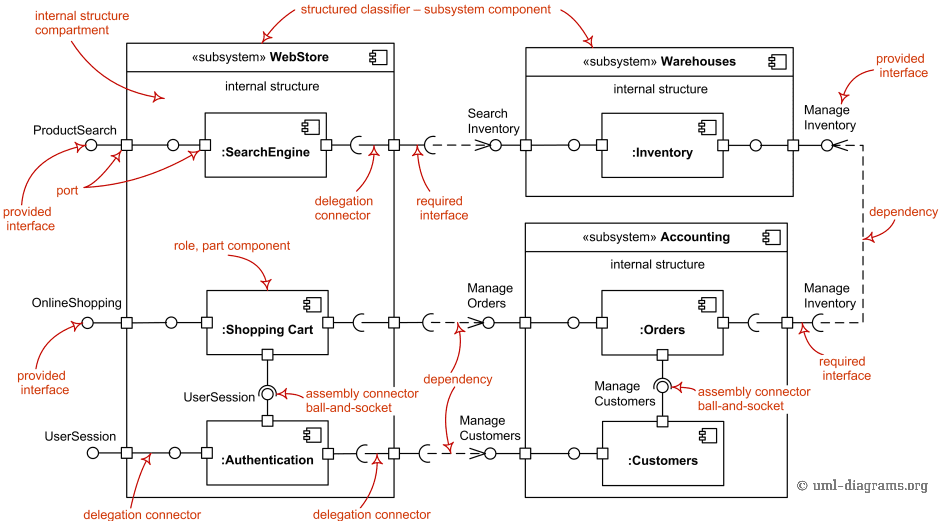
\includegraphics[width=\textwidth]{img/component-diagram.png}
    \caption{Component Diagram.}
\end{figure}

\noindent
To view the component diagram in high resolution, scan (or click) the QR code below.
\begin{center}
    \qrcode{https://github.com/PoliMI-HPC-E-notes-projects-AndreVale69/HPC-E-PoliMI-university-notes/tree/main/software-engineering-for-hpc/notes/img/component-diagram.png}
\end{center}
A complete guide can be found on the following page: \href{https://www.visual-paradigm.com/guide/uml-unified-modeling-language/what-is-component-diagram/}{What is Component Diagram?
}

\newpage

\subsubsection{Sequence Diagram (C\&C structure)}

\definition{Sequence Diagram} show \textbf{elements as they interact over time} and they are organized according to object (horizontally) and time (vertically).

\begin{figure}[!htp]
    \centering
    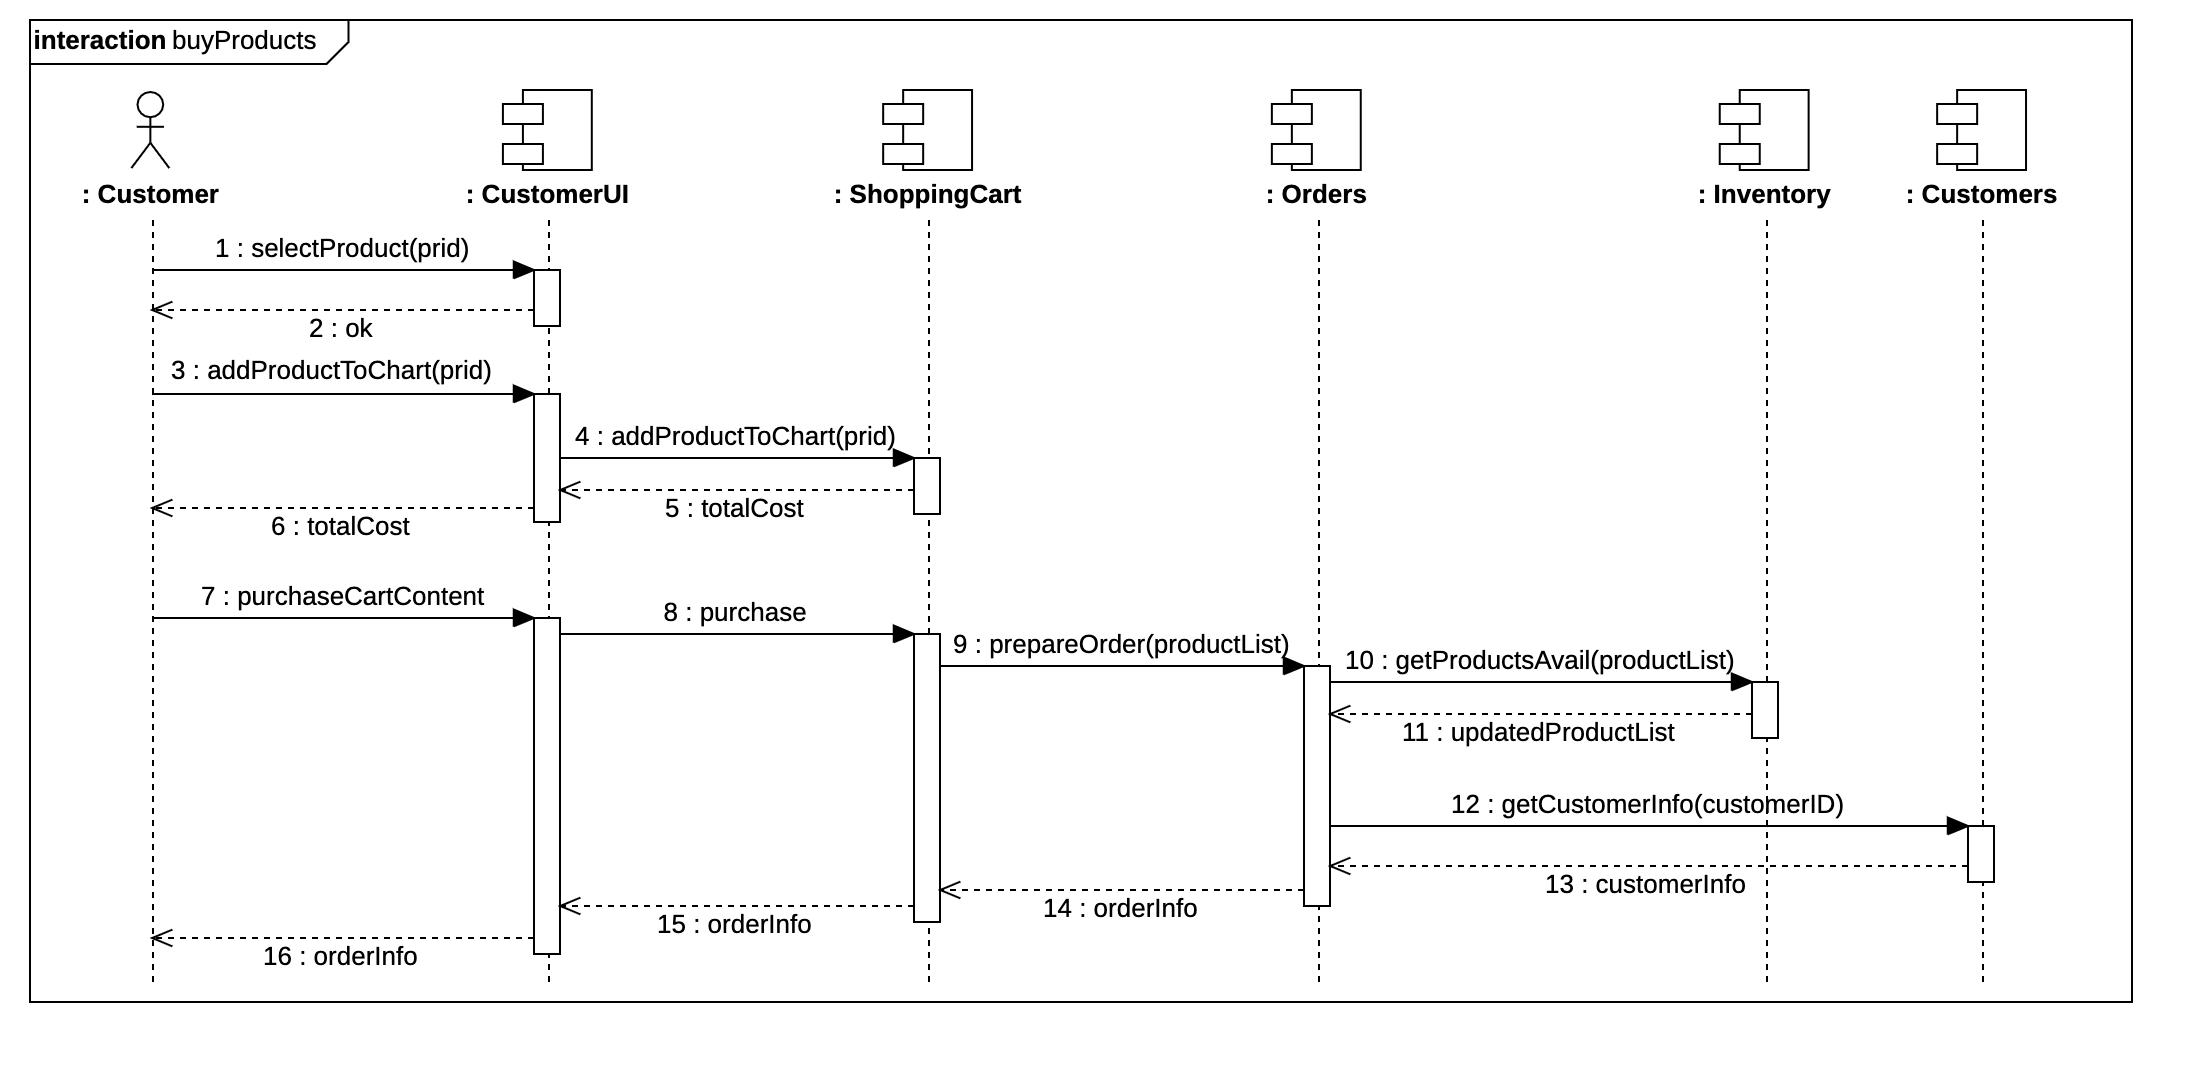
\includegraphics[width=\textwidth]{img/sequence-diagram.png}
    \caption{Sequence Diagram.}
\end{figure}

\noindent
To view the sequence diagram in high resolution, scan (or click) the QR code below.
\begin{center}
    \qrcode{https://github.com/PoliMI-HPC-E-notes-projects-AndreVale69/HPC-E-PoliMI-university-notes/tree/main/software-engineering-for-hpc/notes/img/sequence-diagram.png}
\end{center}
A complete guide can be found on the following page: \href{https://www.visual-paradigm.com/guide/uml-unified-modeling-language/what-is-sequence-diagram/}{What is Sequence Diagram?
}

\newpage

\subsubsection{Class Diagram (module structure)}

A \definition{Class Diagram} is \textbf{a type of static structure diagram} that describes the structure of a system by showing the system's classes, their attributes, operations (or methods), and the relationships among objects.

\begin{figure}[!htp]
    \centering
    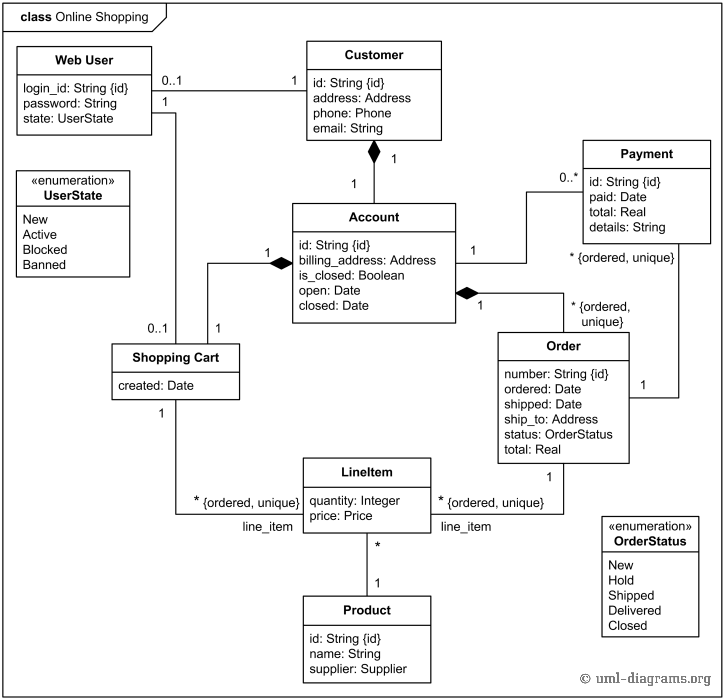
\includegraphics[width=\textwidth]{img/class-diagram.png}
    \caption{Class Diagram.}
\end{figure}

\noindent
To view the sequence diagram in high resolution, scan (or click) the QR code below.
\begin{center}
    \qrcode{https://github.com/PoliMI-HPC-E-notes-projects-AndreVale69/HPC-E-PoliMI-university-notes/tree/main/software-engineering-for-hpc/notes/img/class-diagram.png}
\end{center}
A complete guide can be found on the following page: \href{https://www.visual-paradigm.com/guide/uml-unified-modeling-language/what-is-class-diagram/}{What is Class Diagram?
}

\newpage

\subsubsection{Package Diagram (module structure)}

A \definition{Package Diagram}, a kind of structural diagram, shows the \textbf{arrangement and organization of model elements in middle to large scale project}. Package diagram can show both structure and dependencies between sub-systems or modules, showing different views of a system, for example, as multi-layered (aka multi-tiered) application - multi-layered application model.

\begin{figure}[!htp]
    \centering
    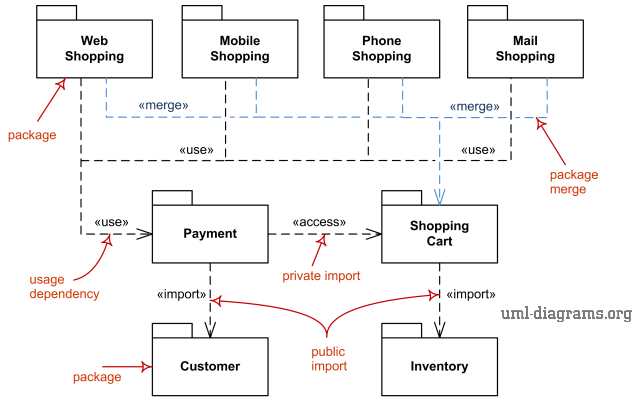
\includegraphics[width=\textwidth]{img/package-diagram.png}
    \caption{Package Diagram.}
\end{figure}

\noindent
To view the sequence diagram in high resolution, scan (or click) the QR code below.
\begin{center}
    \qrcode{https://github.com/PoliMI-HPC-E-notes-projects-AndreVale69/HPC-E-PoliMI-university-notes/tree/main/software-engineering-for-hpc/notes/img/package-diagram.png}
\end{center}
A complete guide can be found on the following page: \href{https://www.visual-paradigm.com/guide/uml-unified-modeling-language/what-is-package-diagram/}{What is Package Diagram?
}

\newpage

\subsubsection{Deployment Diagram (allocation structure)}

A \definition{Deployment Diagram} is a diagram that shows the \textbf{configuration of run time processing nodes and the components that live on them}. Deployment diagrams is a kind of structure diagram used in modeling the physical aspects of an object-oriented system. They are often be used to model the static deployment view of a system (topology of the hardware).

\begin{figure}[!htp]
    \centering
    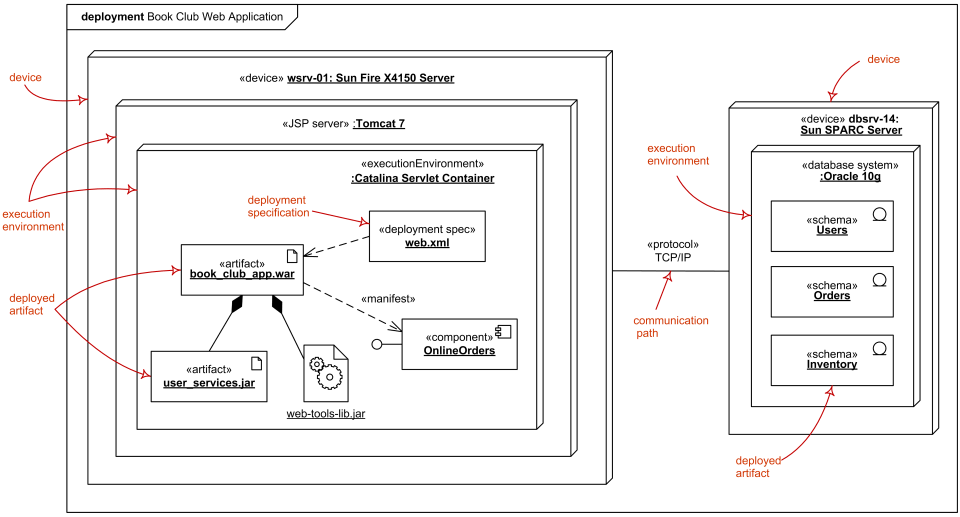
\includegraphics[width=\textwidth]{img/deployment-diagram.png}
    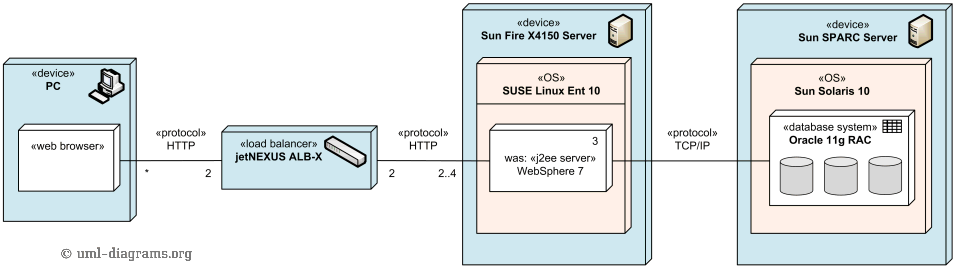
\includegraphics[width=\textwidth]{img/deployment-diagram-2.png}
    \caption{Deployment Diagram.}
\end{figure}

\noindent
To view the sequence diagram in high resolution, scan (or click) the QR code below.
\begin{center}
    \qrcode{https://github.com/PoliMI-HPC-E-notes-projects-AndreVale69/HPC-E-PoliMI-university-notes/tree/main/software-engineering-for-hpc/notes/img/deployment-diagram.png}
    \hspace{2em}
    \qrcode{https://github.com/PoliMI-HPC-E-notes-projects-AndreVale69/HPC-E-PoliMI-university-notes/tree/main/software-engineering-for-hpc/notes/img/deployment-diagram-2.png}
\end{center}
A complete guide can be found on the following page: \href{https://www.visual-paradigm.com/guide/uml-unified-modeling-language/what-is-deployment-diagram/}{What is Deployment Diagram?
}
    \subsection{Design principles}

The following is a list of important design principles in software engineering.

\begin{definitionbox}
    \begin{enumerate}
        \item \textbf{Divide et impera} (also called \emph{divide and conquer})
        
        \item \textbf{Keep the level of abstraction as high as possible}

        \item \textbf{Increase cohesion where possible}

        \item \textbf{Reduce coupling where possible}

        \item \textbf{Design for reusability}

        \item \textbf{Reuse existing designs and code}

        \item \textbf{Design for flexibility}

        \item \textbf{Anticipate obsolescence}

        \item \textbf{Design for portability}

        \item \textbf{Design for testability}

        \item \textbf{Design defensively}
    \end{enumerate}
\end{definitionbox}

\begin{flushleft}
    \large
    \textcolor{Red3}{\textbf{Divide et impera} (\emph{divide and conquer})}
\end{flushleft}
\textbf{Divide and Conquer} is a problem-solving strategy that involves breaking down a complex problem into smaller, more manageable parts, solving each part individually, and then combining the solutions to solve the original problem.

\begin{flushleft}
    \large
    \textcolor{Red3}{\textbf{Keep the level of abstraction as high as possible}}
\end{flushleft}
Ensure that your designs allow you to hide or defer consideration of details, thus reducing complexity. A good abstraction is said to provide \emph{information hiding}. Abstractions allow you to understand the essence of a subsystem without having to know unnecessary details.

    %%%%%%%%%%%%%%%%%%%%%%%
    % Architectural Style %
    %%%%%%%%%%%%%%%%%%%%%%%
    \section{Requirement Engineering}

\subsection{Definition}

Before the definition, we give a possible scenario to understand what requirement engineering is.

\highspace
The municipality of Milan says the following: \dquotes{\emph{The time it takes to make decisions on building permits for residential buildings in the city is too long. We want to develop software that will help us reduce this time}}. So where do we start? How do we identify the most important aspects? How do we make sure that we have understood what our customers want from us?

\begin{definitionbox}
    Software measure engineering (\definition{Requirement Engineering}) is the process of discovering the purpose for which the software is intended by identifying stakeholders and their needs, and documenting these in a form suitable for analysis, communication and subsequent implementation.
\end{definitionbox}

\noindent
The questions derived from requirements engineering are:
\begin{itemize}
    \item Identify stakeholders
    \item Identify their needs
    \item Produce documentation
    \item Analyze, communicate, implement requirements
\end{itemize}

\begin{figure}[!htp]
    \centering
    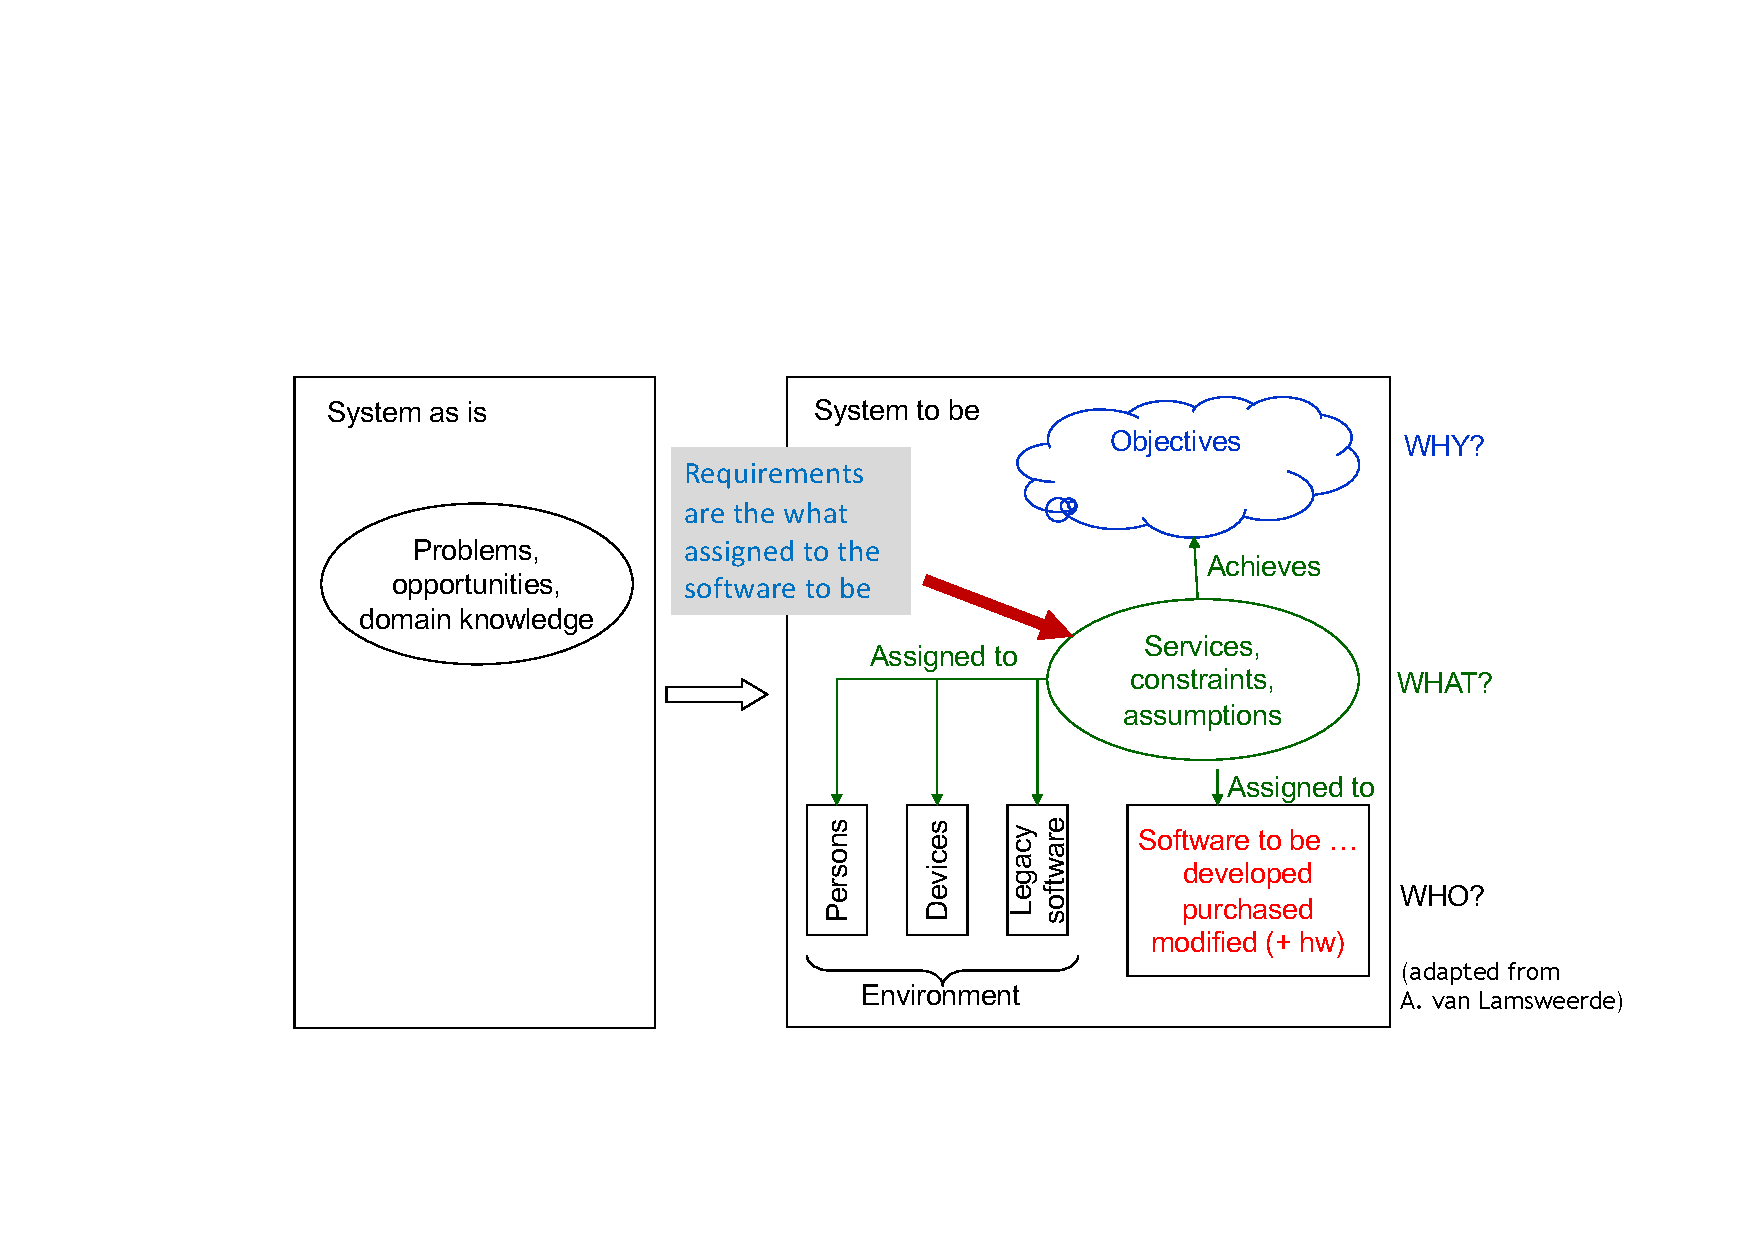
\includegraphics[width=\textwidth]{img/requirement-engineering-1.pdf}
    \caption{Analyzing the system as is and the system to be.}
\end{figure}
    \subsection{Client-Server}

A \definition{Client-Server Architecture} is a \textbf{network-based computing structure} where responsibilities and operations get \textbf{distributed between clients and servers}. Client-Server Architecture is widely used for network applications such as email, web, online banking, e-commerce, etc.

\begin{flushleft}
    \textcolor{Green3}{\textbf{\faIcon{check} When to use it}}
\end{flushleft}
The three most common cases are:
\begin{itemize}
    \item When \textbf{multiple users} need to access a \textbf{single resource} (e.g. database).

    \item When there is a preexisting software and we must \textbf{access remotely} (e.g. email server).
    
    \item When it is convenient to organize the system around a \textbf{shared piece of functionality used by multiple components} (e.g. authentication or authorization server).
\end{itemize}

\begin{flushleft}
    \textcolor{Red2}{\textbf{\faIcon{exclamation-triangle} Technical issues}}
\end{flushleft}
With this architecture, it's necessary to \textbf{design} and \textbf{document} proper \textbf{interfaces} for our server. It is also necessary to ensure that the server can \textbf{handle multiple simultaneous requests}.

\subsubsection{Interface design}

An \definition{interface design} is a \textbf{boundary} across which components interact. Proper definition of interfaces is an architectural concern (affects maintainability, usability, testability, performance, integrability). There are two important \textbf{guiding principles} for interface design: \textbf{information hiding} and \textbf{low coupling}. An interface should encapsulate a component implementation so that it can be changed without affecting other components.

\highspace
There are several aspects to interface design that need to be considered:
\begin{itemize}
    \item \definition{Contract principle}: any resource (operation, data) added to an interface implies a \textbf{commitment to maintaining} it.

    \item \definition{Least surprise principle}: interfaces should \textbf{behave} consistently \textbf{with expectations}.

    \item \definition{Small interfaces principle}: interfaces should limit the \textbf{exposed resources to the minimum}.
\end{itemize}
There are also some important elements to define: \textbf{interaction style} (e.g. sockets, RPC, REST); \textbf{representation} and structure of exchanged data (affecting expressiveness, interoperability, performance and transparency); \textbf{error handling}.

\newpage

\subsubsection{Error handling, multiple interfaces and interface evolution}

Sometimes there may be some problems, for example: an operation is called with invalid parameters and consequently the call doesn't return anything. This simple example can provoke some scenarios: the component cannot handle the request in its current state; or hardware/software errors prevent successful execution; or there is a misconfiguration issue (e.g. the server is not correctly connected to the database).

There are three possible \textbf{solutions}: \textbf{raising an exception}; \textbf{return an error code} (common); \textbf{log the problem}. There's no single solution, but we can choose several (e.g. error code and log the problem).

\highspace
A \textbf{server} can offer \definition{multiple interfaces} at the same time. This enables separation of concerns, different levels of access rights and support ot \textbf{interface evolution}.

\highspace
\textbf{Interface evolution} occurs for many reasons (e.g. to support new requirements). Several \textbf{strategies} are needed to support continuity:
\begin{itemize}
    \item \textbf{\underline{Deprecation}}: declare well in advance that an interface version will be retired by a certain date;

    \item \textbf{\underline{Versioning}}: maintain multiple active versions of the interface;

    \item \textbf{\underline{Extension}}: a new version extends the previous one.
\end{itemize}

\newpage

\subsubsection{Handling multiple requests}

The server must be able to receive and process requests from multiple clients. There are two main approaches to this: \emph{forking} and \emph{worker pooling}.

\begin{flushleft}
    \large
    \textcolor{Red2}{\textbf{Forking}}
\end{flushleft}
The \definition{forking} approach is the same as that used by the Apache Web Server: \textbf{one process per request or per client}.

\begin{figure}[!htp]
    \centering
    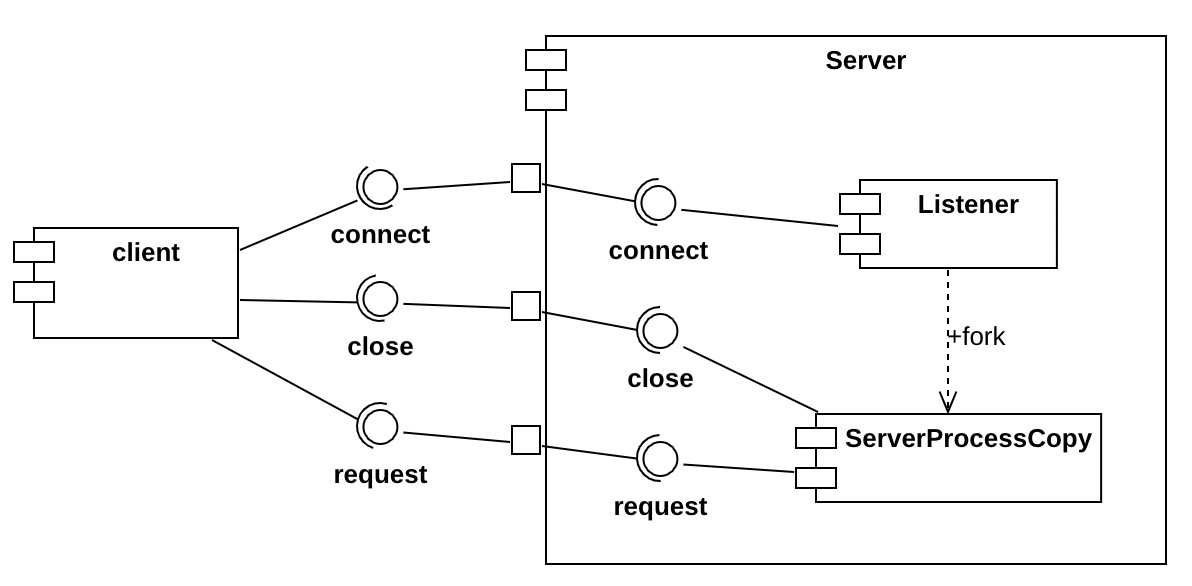
\includegraphics[width=.8\textwidth]{img/forking-1.png}
    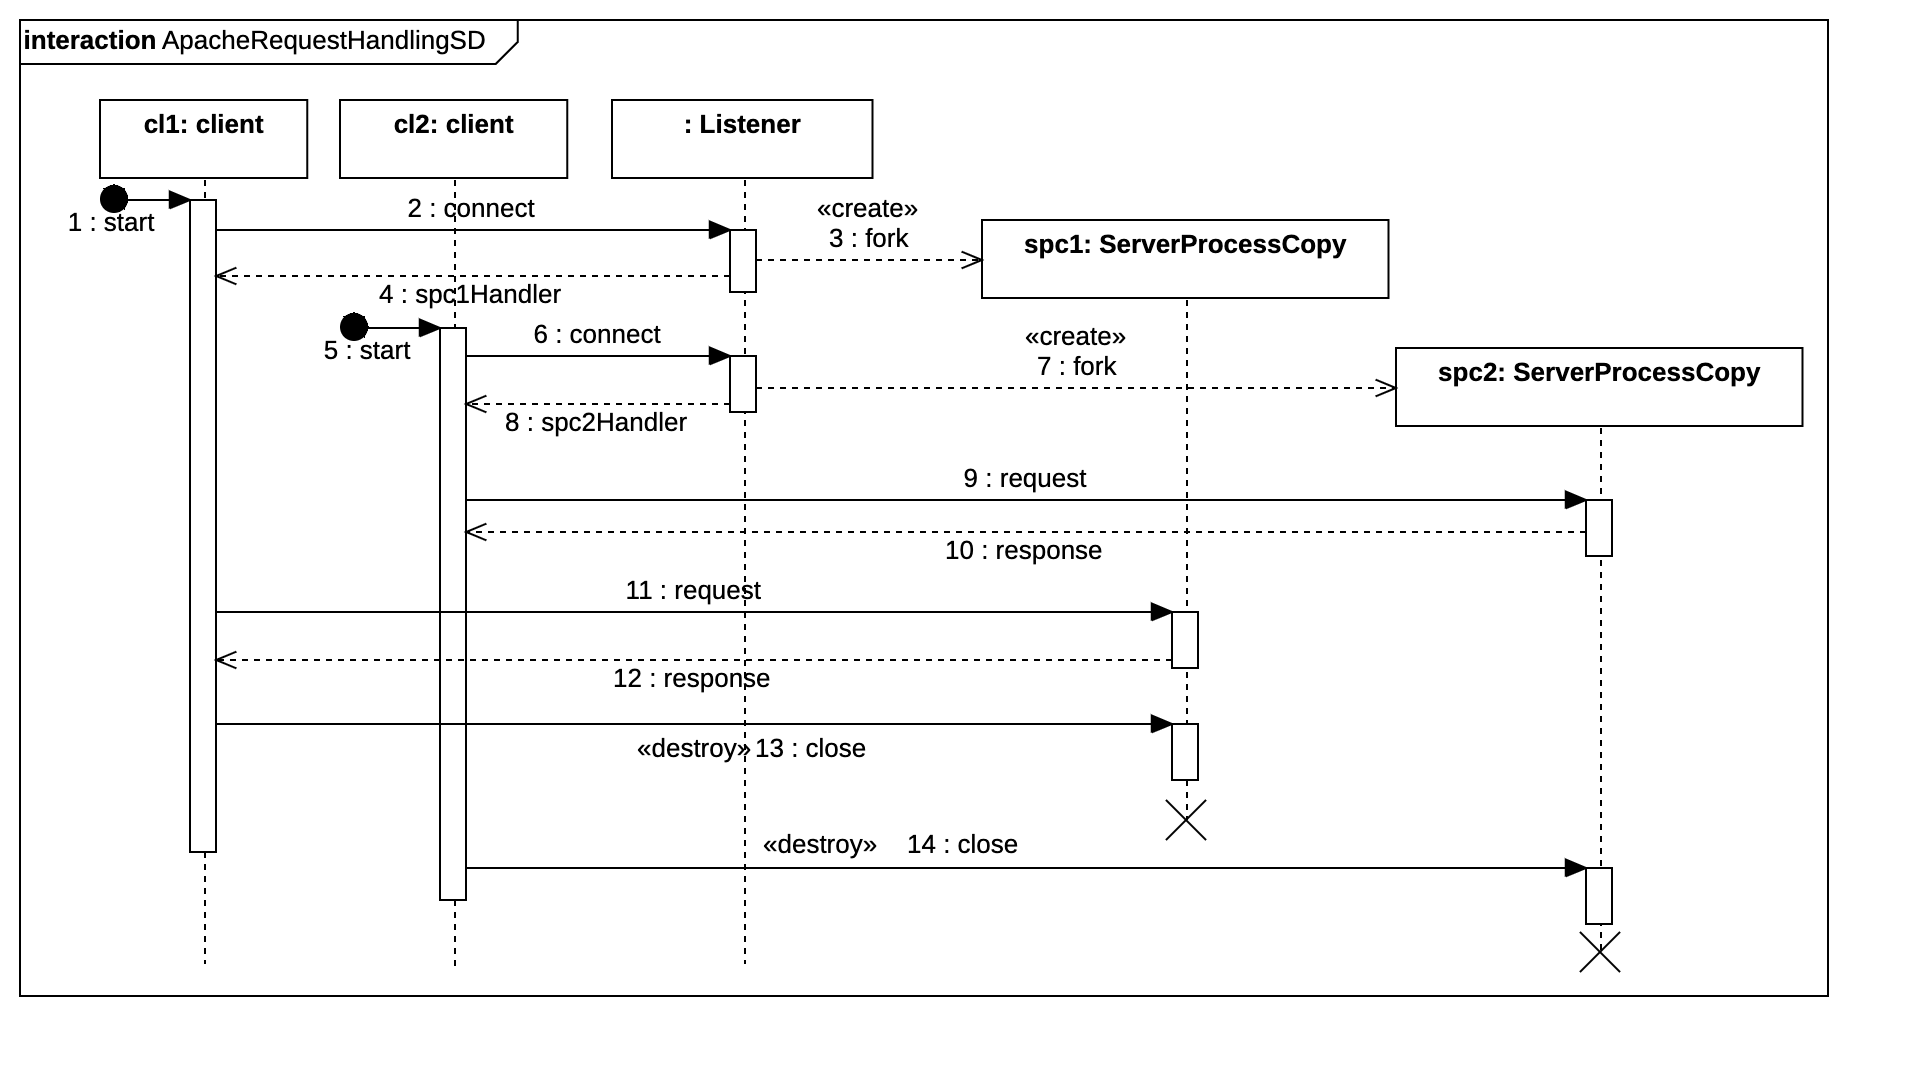
\includegraphics[width=\textwidth]{img/forking-2.png}
    \caption{Forking diagrams.}
\end{figure}

\begin{flushleft}
    \textcolor{Green3}{\textbf{\faIcon{check} Forking Advantages}}
\end{flushleft}
\begin{itemize}
    \item Architectural \textbf{simplicity}.
    
    \item \textbf{Isolation} and \textbf{protection} given by the one-connection-per-process model. Note: slow processes do not affect other incoming connections.
    
    \item \textbf{Simple to program}.
\end{itemize}

\newpage

\begin{flushleft}
    \textcolor{Red2}{\textbf{\faIcon{exclamation-triangle} Forking Issues}}
\end{flushleft}
\begin{itemize}
    \item Growth of the WWW over the last 20 years (number of users and weight of web pages).
    
    \item The number of \textbf{active processes} at time $t$ is \textbf{difficult to predict} and may \textbf{saturate resources}.
    
    \item \textbf{Expensive} fork-kill operations for each \textbf{incoming connection}.
\end{itemize}

\newpage

\begin{flushleft}
    \large
    \textcolor{Red2}{\textbf{Worker pooling}}
\end{flushleft}
It is an alternative approach adopted by NGINX Web Server. It is \textbf{designed for high concurrency} but has to deal with \textbf{scalability issues}.

\begin{figure}[!htp]
    \centering
    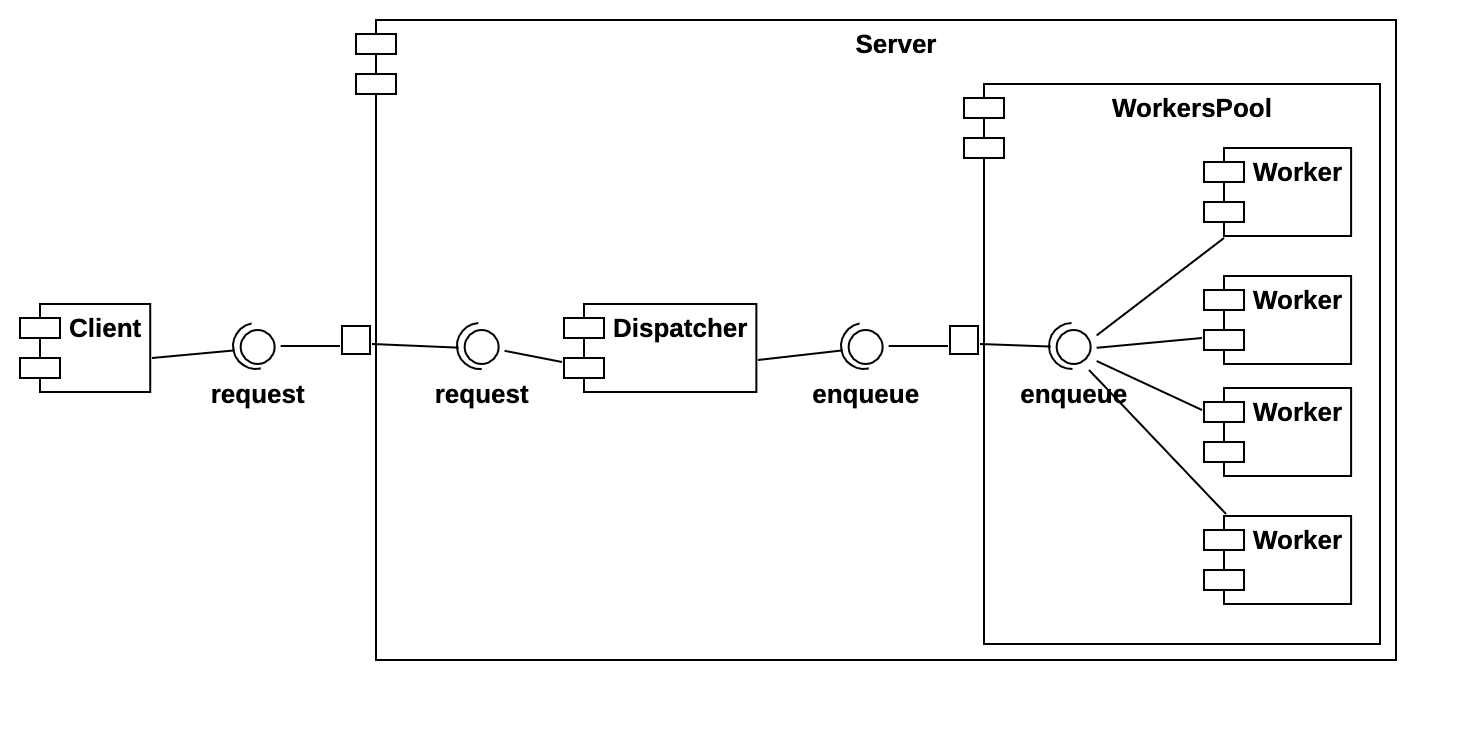
\includegraphics[width=.9\textwidth]{img/worker-pooling-1.png}
    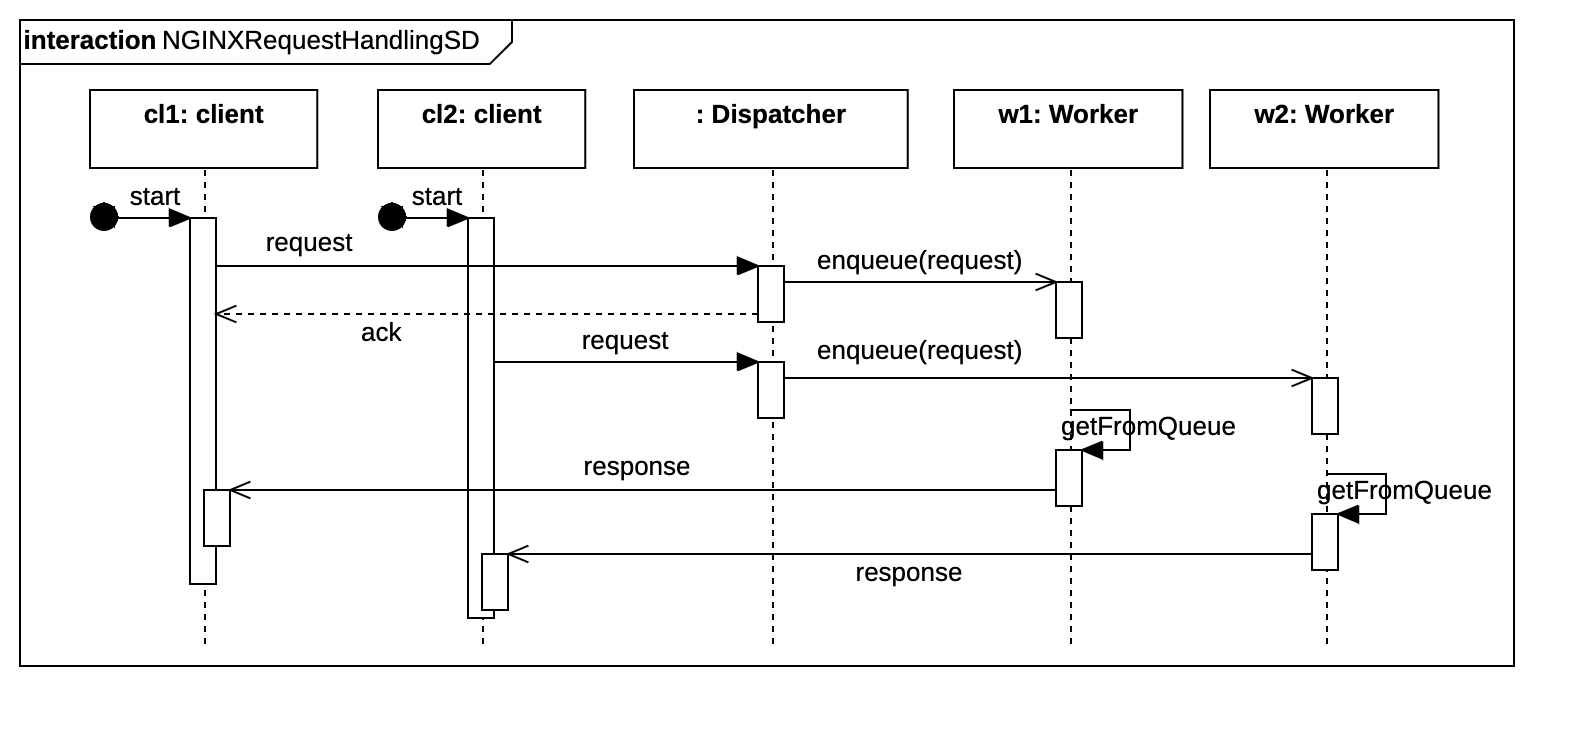
\includegraphics[width=\textwidth]{img/worker-pooling-2.png}
    \caption{Worker pooling diagrams.}
\end{figure}

\noindent
Despite the well-known problem of this architecture (scalability), NGINX addresses the previous problems by introducing a new \textbf{architectural tactic}. A \emph{tactic} is a \textbf{design decision that affects the control of one or more quality attributes}.

\begin{flushleft}
    \textcolor{Green3}{\textbf{\faIcon{check} Worker Pooling Advantages (quality attribute trade-offs)}}
\end{flushleft}
\begin{itemize}
    \item Number of \textbf{workers} is fixed, so they \textbf{do not saturate available resources}.
    
    \item \textbf{Each worker} has a \textbf{queue}.
    
    \item When \textbf{queues} are \textbf{full} the \textbf{dispatcher drops the incoming requests} to keep high performance (\textbf{optimize scalability and performance by sacrificing availability}).
    
    \item Dispatcher \textbf{balances} the \textbf{workload} among available workers \textbf{according to specific policies}.
\end{itemize}
    \subsection{Three-Tier Architecture}

The following is a summary of the \href{https://www.ibm.com/topics/three-tier-architecture}{IBM guide}.

\highspace
\definition{Three-tier architecture} is a well-established software application architecture that \textbf{organizes applications into three logical and physical computing tiers}: 
\begin{itemize}
    \item The \textbf{presentation} tier, or user interface;
    
    \item The \textbf{application} tier, where data is processed;
    
    \item The \textbf{data} tier, where application data is stored and managed.
\end{itemize}

\begin{flushleft}
    \textcolor{Green3}{\textbf{\faIcon{check} Benefits}}
\end{flushleft}
The chief benefit of three-tier architecture is its \textbf{logical and physical separation} of functionality. Each tier can run on a separate operating system and server platform - for example, web server, application server, database server - that best fits its functional requirements. And each tier runs on at least one dedicated server hardware or virtual server, so the services of \textbf{each tier can be customized and optimized without impacting the other tiers}. Other benefits include:
\begin{itemize}
    \item \textbf{Faster development}: Because \emph{each tier can be developed simultaneously by different teams}, an organization can bring the application to market faster. And programmers can use the latest and best languages and tools for each tier.
    
    \item \textbf{Improved scalability}: \emph{Any tier can be scaled independently} of the others as needed.

    \item \textbf{Improved reliability}: An outage in one tier is less likely to impact the availability or performance of the other tiers.

    \item \textbf{Improved security}: Because the \emph{presentation tier and data tier can't communicate directly}, a well-designed application tier can function as an internal firewall, preventing SQL injections and other malicious exploits.
\end{itemize}

\subsubsection{N-tier architecture}

\definition{N-tier architecture} (also called or multitier architecture) refers to any application architecture with \textbf{more than one tier}. But applications with more than three layers are \underline{rare} because extra layers offer \textbf{few benefits} and can make the \textbf{application slower}, \textbf{harder to manage} and \textbf{more expensive to run}. As a result, n-tier architecture and multitier architecture are usually synonyms for three-tier architecture.
    \subsection{Microservice architectural style}

The microservice architectural style is an approach to developing a single application as a suite of \textbf{small services}, each running in its own process and communicating \textbf{lightweight mechanisms}, often an HTTP resource API.

\begin{flushleft}
    \textcolor{Green3}{\textbf{\faIcon{check} Benefits}}
\end{flushleft}
There are two main benefits:
\begin{itemize}
    \item \textbf{Technology heterogeneity}. \textbf{Each service uses its own technology stack}. The technology stack can be selected to fit the task best (e.g. data analysis vs video streaming). The teams can experiment with new technologies within a single microservice (e.g. we can deploy two versions and do A/B testing). Also, no unnecessary dependencies or libraries for each service.
    
    \item \textbf{Scaling}. \textbf{Each microservice can be scaled independently}. Also, identified bottlenecks can be addressed directly. Parts of the system that do not represent bottlenecks can remain simple and unscaled.
\end{itemize}
    \subsection{Event-Driven Architecture}

An \definition{Event-Driven Architecture} uses \textbf{events to trigger and communicate between decoupled services} and is common in modern applications built with microservices. An event is a change in state, or an update, like an item being placed in a shopping cart on an e-commerce website. Events can either carry the state (the item purchased, its price, and a delivery address) or events can be identifiers (a notification that an order was shipped).

Often it's called \textbf{publish-subscribe} (publish is the event generation, and subscribe is the declaration of the interest).

\begin{flushleft}
    \textcolor{Green3}{\textbf{\faIcon{check} Benefits}}
\end{flushleft}
\begin{itemize}
    \item \textbf{Very common in modern development practices} (e.g. continuous integration and deployment, such as GitHub Actions).

    \item \textbf{Easy addition/deletion of components} (publishers and subscribers are decoupled; the event dispatcher handles this dynamic set).
\end{itemize}

\begin{flushleft}
    \textcolor{Red2}{\textbf{\faIcon{exclamation-triangle} Problems}}
\end{flushleft}
\begin{itemize}
    \item \textbf{Potential scalability problems} (the event dispatcher may become a bottleneck under high workload).
    
    \item \textbf{Ordering of events} (not guaranteed, not straightforward).
\end{itemize}

\highspace
Other characteristics of this architecture:
\begin{itemize}
    \item THe messages and the events are \textbf{asynchronous}.
    
    \item Computation is \textbf{reactive} (driven by receipt of message).

    \item \textbf{Destination} of messages \textbf{determined by receiver}, not sender (location/identity abstraction).

    \item \textbf{Loose coupling} (senders and receivers added without reconfiguration).
    
    \item \textbf{Flexible} communication means (one-to-many, many-to-one, many-to-many).
\end{itemize}
Some \example{examples} of relevant technologies are: \href{https://kafka.apache.org/}{Apache Kafka} and \href{https://www.rabbitmq.com/}{RabbitMQ}.

\newpage

\subsubsection{Apache Kafka}

\definition{Kafka} is a \textbf{framework} for the event-driven paradigm:
\begin{itemize}
    \item Includes primitives to create \textbf{event produces} and \textbf{consumers} and a runtime infrastructure to handle \textbf{event transfer} from producers to consumers.
    
    \item \textbf{Stores events} durably and reliably.
    
    \item Allow consumers to \textbf{process events} as they occur or retrospectively.
\end{itemize}
These services are offered in a distributed, highly scalable, elastic, fault-tolerant, and secure manner.

\begin{figure}[!htp]
    \centering
    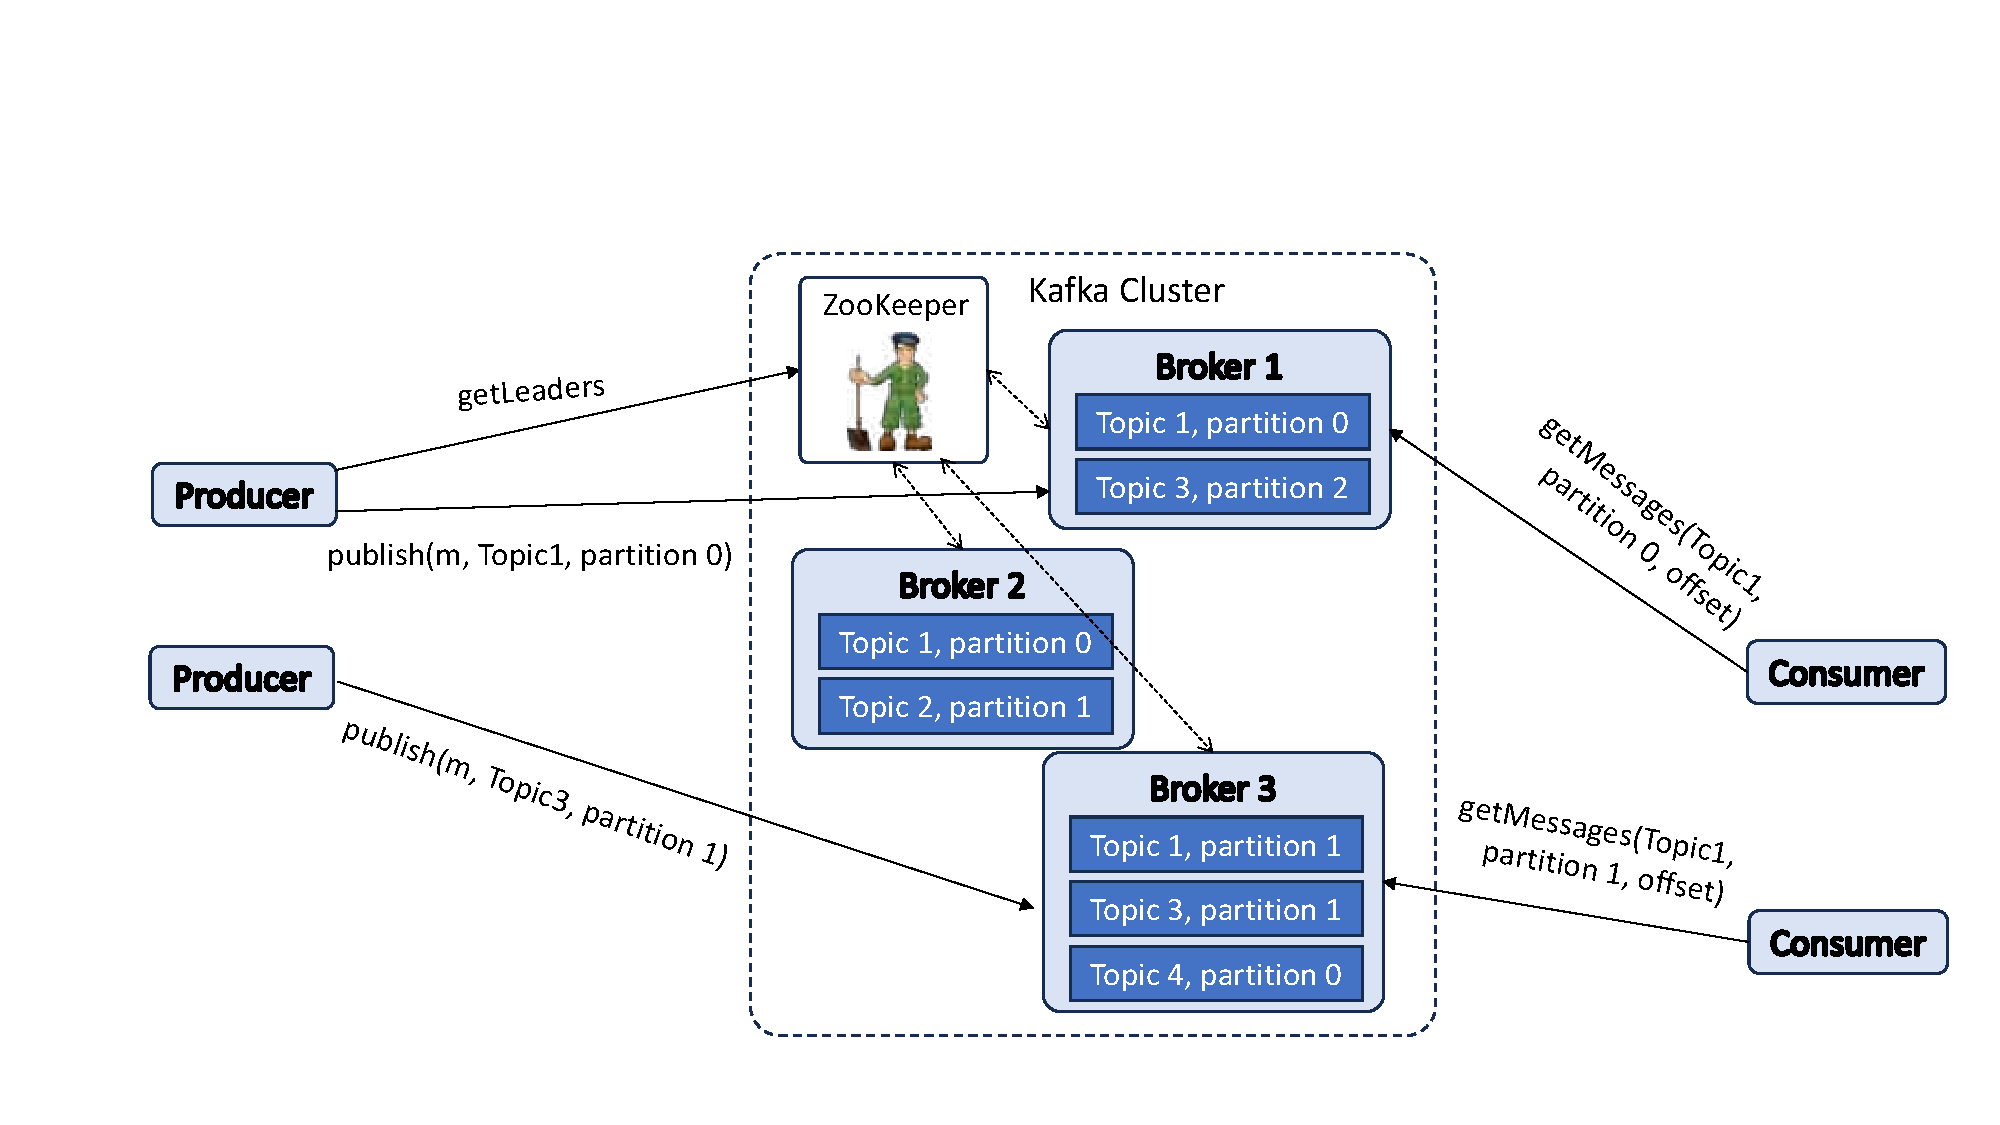
\includegraphics[width=\textwidth]{img/kafka-arch-1.pdf}
    \caption{Kafka architecture (the ZooKeeper is a \dquotes{health manager}).}
\end{figure}

\noindent
Some important features:
\begin{itemize}
    \item Each \textbf{broker} handles a set of \textbf{topics} and \textbf{topic partitions}, parts including sets of messages on the topic.

    \item The \emph{partitions} are independent from each other and can be \textbf{replicated} on multiple brokers for fault tolerance.

    \item There is \textbf{one leading broker per partition}. The other brokers containing the same partition are \textbf{followers}.
    
    \item The \textbf{producers} know the available leading brokers and send messages to them.
    
    \item \textbf{Messages in the same topic} are organized in \textbf{batches} at the producers' side and then sent to the broker when the batch size overcomes a certain threshold.

    \item \textbf{Consumers} adopt a \textbf{pull approach}. They \emph{receive in a single batch all messages} belonging to a certain partition starting from a specified offset.

    \item \textbf{Messages} remain \textbf{available} at the brokers' side \textbf{for a specified period} and can be \textbf{read multiple times} in this period.
    
    \item The leader keeps track of the \textbf{in-synch followers}.
    
    \item \textbf{ZooKeeper is used to monitor the correct operation of the cluster}. All brokers send heartbeats to ZooKeeper. ZooKeeper will replace a failed broker by electing a new leader for all partitions that the failed broker was leading. It can also start/restart brokers.
\end{itemize}

\begin{center}
    \large
    \textcolor{Red2}{\textbf{Message delivery}}
\end{center}

\begin{flushleft}
    \textcolor{Red2}{\textbf{Producer}}
\end{flushleft}
\begin{enumerate}
    \item Brokers commit messages by storing them in the corresponding partition;
    
    \item Leader adds the message to followers (replicas) if available.
\end{enumerate}

\begin{figure}[!htp]
    \centering
    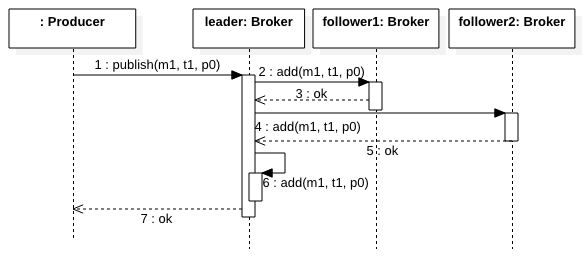
\includegraphics[width=\textwidth]{img/kafka-producer.png}
    \caption{Sequence diagram Kafka producer.}
\end{figure}

\noindent
A possible \textbf{issue}: in case of failure, the \textbf{producer may not get the response} (message number 7 in figure). In this case, the producer has to resend the message and kafka brokers can identify and eliminate duplicates.

\highspace
Synchronization with replicas can be transactional and it's possible to choose between the following options:
\begin{itemize}
    \item \textbf{Exactly-once} semantics is possible but long waiting time. So \textbf{replicas are not allowed}, but the problem is that Kafka spent a \textbf{long time trying to guarantee uniqueness}.

    \item \textbf{At-least-once} can be chosen by excluding duplicates' management.

    \item \textbf{At-most-once} can be chosen by publishing messages asynchronously.
\end{itemize}

\begin{flushleft}
    \textcolor{Red2}{\textbf{Consumer}}
\end{flushleft}
Each \textbf{consumer} can rely on a \textbf{persistent log} to keep track of the \textbf{offset} so that it is not lost in case of failure.

\highspace
\textbf{Issue} case: if the consumer fails after having elaborated messages and before storing the new offset in the log, the same messages will be retrieved again (\textbf{at-least-once semantics}). Note that the delivery semantics can be changed if the new offset is store before the elaboration and we can choose \textbf{at-most-once semantics} because, if failing after storing the offset, the effect of the received messages does not materialize. Finally, transactional management of the log also allows for \textbf{exactly-once semantics}.

\begin{figure}[!htp]
    \centering
    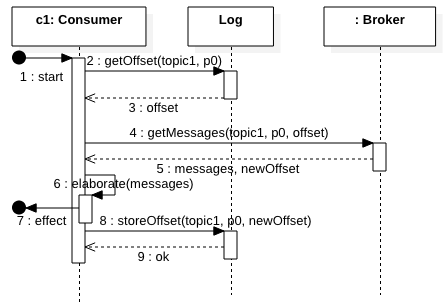
\includegraphics[width=.8\textwidth]{img/kafka-consumer.png}
    \caption{Sequence diagram Kafka consumer.}
\end{figure}

\begin{center}
    \large
    \textcolor{Red2}{\textbf{Kafka architectural tactics}}
\end{center}
There are some tactics used to improve some features of Kafka. In the following section we can see scalability and fault tolerance.

\begin{flushleft}
    \textcolor{Red2}{\textbf{Improve Scalability}}
\end{flushleft}
By \textbf{creating multiple partitions and multiple brokers}, we can create the ability to distribute producers/consumers to different partitions handled by different brokers. We can also \textbf{scale the operations} because Kafka supports the \textbf{creation of clusters of brokers}. Consider that each cluster contains up to a hundred brokers capable of handling trillions of messages per day.

\begin{flushleft}
    \textcolor{Red2}{\textbf{Improve Fault Tolerance}}
\end{flushleft}
By \textbf{creating partitions}, we use the \textbf{persistence} of the partitions. \textbf{Replication} also reduces the risk of data loss. Finally, cluster management takes care of restarting brokers and setting leaders as needed.

    %%%%%%%%%%%%%%%%%%%%%%%%%%
    % Bibliography and index %
    %%%%%%%%%%%%%%%%%%%%%%%%%%
    \bibliography{bibtex}{}
\bibliographystyle{plain}

\newpage

\printindex
\end{document}